%Version 3.1 December 2024
% See section 11 of the User Manual for version history
%
%%%%%%%%%%%%%%%%%%%%%%%%%%%%%%%%%%%%%%%%%%%%%%%%%%%%%%%%%%%%%%%%%%%%%%
%%                                                                 %%
%% Please do not use \input to include other tex files.       %%
%% Submit your LaTeX manuscript as one .tex document.              %%
%%                                                                 %%
%% All additional figures and files should be attached             %%
%% separately and not embedded in the \TeX\ document itself.       %%
%%                                                                 %%
%%%%%%%%%%%%%%%%%%%%%%%%%%%%%%%%%%%%%%%%%%%%%%%%%%%%%%%%%%%%%%%%%%%%%

%%\documentclass[referee,sn-basic]{sn-jnl}% referee option is meant for double line spacing

%%=======================================================%%
%% to print line numbers in the margin use lineno option %%
%%=======================================================%%

%%\documentclass[lineno,pdflatex,sn-basic]{sn-jnl}% Basic Springer Nature Reference Style/Chemistry Reference Style

%%=========================================================================================%%
%% the documentclass is set to pdflatex as default. You can delete it if not appropriate.  %%
%%=========================================================================================%%

%%\documentclass[sn-basic]{sn-jnl}% Basic Springer Nature Reference Style/Chemistry Reference Style

%%Note: the following reference styles support Namedate and Numbered referencing. By default the style follows the most common style. To switch between the options you can add or remove “Numbered” in the optional parenthesis.
%%The option is available for: sn-basic.bst, sn-chicago.bst%

%%\documentclass[pdflatex,sn-nature]{sn-jnl}% Style for submissions to Nature Portfolio journals
%%\documentclass[pdflatex,sn-basic]{sn-jnl}% Basic Springer Nature Reference Style/Chemistry Reference Style
\documentclass[pdflatex,sn-mathphys-ay]{sn-jnl}% Math and Physical Sciences Author Year Reference Style
%%\documentclass[pdflatex,sn-aps]{sn-jnl}% American Physical Society (APS) Reference Style
%%\documentclass[pdflatex,sn-vancouver-num]{sn-jnl}% Vancouver Numbered Reference Style
%%\documentclass[pdflatex,sn-vancouver-ay]{sn-jnl}% Vancouver Author Year Reference Style
%%\documentclass[pdflatex,sn-apa]{sn-jnl}% APA Reference Style
%%\documentclass[pdflatex,sn-chicago]{sn-jnl}% Chicago-based Humanities Reference Style

%%%% Standard Packages
%%<additional latex packages if required can be included here>

\usepackage{graphicx}%
\usepackage{multirow}%
\usepackage{amsmath,amssymb,amsfonts}%
\usepackage{amsthm}%
\usepackage{xcolor}%
\usepackage{textcomp}%
\usepackage{manyfoot}%
\usepackage{booktabs}%
\usepackage{longtable}%
\usepackage{tabularx}%
\usepackage{algorithm}%
\usepackage{algorithmicx}%
\usepackage{algpseudocode}%
\usepackage{listings}%
\usepackage{float}%
\usepackage{pdflscape}%
\usepackage[section]{placeins}%
%%%%

%%%%%=============================================================================%%%%
%%%%  Remarks: This template is provided to aid authors with the preparation
%%%%  of original research articles intended for submission to journals published
%%%%  by Springer Nature. The guidance has been prepared in partnership with
%%%%  production teams to conform to Springer Nature technical requirements.
%%%%  Editorial and presentation requirements differ among journal portfolios and
%%%%  research disciplines. You may find sections in this template are irrelevant
%%%%  to your work and are empowered to omit any such section if allowed by the
%%%%  journal you intend to submit to. The submission guidelines and policies
%%%%  of the journal take precedence. A detailed User Manual is available in the
%%%%  template package for technical guidance.
%%%%%=============================================================================%%%%

%% as per the requirement new theorem styles can be included as shown below
\theoremstyle{thmstyleone}%
\newtheorem{theorem}{Theorem}%  meant for continuous numbers
\newtheorem{proposition}[theorem]{Proposition}%

\theoremstyle{thmstyletwo}%
\newtheorem{example}{Example}%
\newtheorem{remark}{Remark}%

\theoremstyle{thmstylethree}%
\newtheorem{definition}{Definition}%

\raggedbottom
\setcounter{topnumber}{3}
\setcounter{dbltopnumber}{3}
\renewcommand{\topfraction}{0.9}
\renewcommand{\dbltopfraction}{0.9}
\renewcommand{\textfraction}{0.08}
\renewcommand{\floatpagefraction}{0.8}
\renewcommand{\dblfloatpagefraction}{0.8}
\setlength{\LTleft}{0pt}
\setlength{\LTright}{0pt}
\hypersetup{hypertexnames=false}
%%\unnumbered% uncomment this for unnumbered level heads

\begin{document}

\title[IVF/SPEA2]{A Budget-Controlled In Vitro Fertilization Memetic Hybrid for SPEA2 on Bi- and Tri-Objective Problems}

%%=============================================================%%
%% GivenName	-> \fnm{Joergen W.}
%% Particle	-> \spfx{van der} -> surname prefix
%% FamilyName	-> \sur{Ploeg}
%% Suffix	-> \sfx{IV}
%% \author*[1,2]{\fnm{Joergen W.} \spfx{van der} \sur{Ploeg}
%%  \sfx{IV}}\email{iauthor@gmail.com}
%%=============================================================%%

\author*[1]{\fnm{Pedro Sanches} \sur{Zambrano}}\email{pedrosanches@discente.ufg.br}
%% TODO: Add ORCID iDs in the submission portal (guidelines require at least the corresponding author's ORCID)

\author[1]{\fnm{Eduardo Faria} \spfx{de} \sur{Souza}}

\author[1]{\fnm{Altino} \sur{Dantas}}

\author[1]{\fnm{S\'avio Menezes} \sur{Sampaio}}

\author[1]{\fnm{Celso G.} \sur{Camilo-Junior}}

\affil*[1]{\orgdiv{Institute of Informatics}, \orgname{Federal University of Goi\'as}, \orgaddress{\street{Avenida Esperan\c{c}a, s/n, Campus Samambaia}, \city{Goi\^ania}, \postcode{74690-900}, \state{GO}, \country{Brazil}}}

\abstract{%
	The Strength Pareto Evolutionary Algorithm 2 (SPEA2) remains a standard baseline in multiobjective optimization, but its density-based truncation can remove offspring generated by local intensification. We study a budget-controlled memetic hybrid that inserts an in vitro fertilization phase into SPEA2 while preserving the host's generation-level evaluation budget. The implementation analyzed here combines dissimilar-father selection with a collective cycle-continuation rule so that intensification is retained only when it improves the population under SPEA2's archive dynamics. A three-phase tuning pipeline on 12 representative problem-objective configurations defines the default setting. The resulting method is evaluated on 39 out-of-sample synthetic instances, the full 51-instance synthetic suite, and three constrained engineering problems. Against canonical SPEA2 over 60 runs per configuration, the method achieves Holm--Bonferroni-corrected inverted generational distance win/loss/tie counts of 19/2/3 on out-of-sample bi-objective instances and 12/0/3 on out-of-sample tri-objective instances; on the full synthetic suite the corresponding counts are 22/3/3 and 15/1/7. Hypervolume provides secondary support. Improvements concentrate on regular Pareto-front geometries, whereas disconnected or irregular fronts can weaken or reverse the effect because intensification-generated density interacts unfavorably with SPEA2 truncation. The results therefore support a conditional, host-specific memetic improvement over SPEA2 at moderate objective counts rather than a universal replacement.%
}

\keywords{memetic computing, strength Pareto evolutionary algorithm 2, in vitro fertilization, multiobjective optimization, Pareto-front geometry}

\maketitle

\section{Introduction}\label{sec1}

A multi-objective optimization problem can be written as
\[
	\min_{\mathbf{x}\in\Omega}\ \mathbf{f}(\mathbf{x}) = \bigl(f_1(\mathbf{x}),\ldots,f_M(\mathbf{x})\bigr),
\]
where $\Omega \subseteq \mathbb{R}^D$ is the decision space. The Pareto set $P$ contains the non-dominated decision vectors, and its image $PF = \{\mathbf{f}(\mathbf{x}) \mid \mathbf{x}\in P\}$ is the Pareto front. Evolutionary multi-objective algorithms (MOEAs) such as the Nondominated Sorting Genetic Algorithm II (NSGA-II) \citep{deb2002fast}, the Multiobjective Evolutionary Algorithm based on Decomposition (MOEA/D) \citep{zhang2007moead}, and the Strength Pareto Evolutionary Algorithm 2 (SPEA2) \citep{zitzler2001spea2} are a standard class of methods for approximating $PF$ \citep{zhou2011multiobjective}. Among them, SPEA2 remains an important baseline and a natural hybridization host because it combines elitist archiving, dominance-based fitness assignment, and nearest-neighbor density estimation in a compact environmental-selection framework.

In SPEA2, however, bounded-archive maintenance and density-based diversity control introduce an explicit convergence--spread trade-off on irregular Pareto-front geometries. Analyses of adaptive archiving and proximity--diversity balance show that maintaining a well-distributed approximation can conflict with pure proximity improvement, especially on irregular or disconnected fronts \citep{knowles2003properties, bosman2003balance}. As the number of objectives grows, this trade-off becomes more acute because a larger fraction of the population is non-dominated and density-related selection effects become increasingly influential \citep{ishibuchi2008evolutionary, li2015many}. This broader pressure motivated density-oriented refinements such as shift-based estimation \citep{li2014shift}. We therefore focus on the bi-objective ($M=2$) and tri-objective ($M=3$) regimes, where dominance still exerts useful pressure but density-induced stagnation remains practically relevant.

Memetic algorithms address such limitations by embedding problem-focused intensification into evolutionary search. The in vitro fertilization (IVF) procedure is a biologically inspired population-based intensification method \citep{camilo-junior2011} that has already been coupled with MOEAs such as NSGA-II \citep{sampaio2017ivf} and the Nondominated Sorting Genetic Algorithm III (NSGA-III) \citep{Sampaio2024}. In memetic-computing terms, IVF is not merely an additional variation operator: it is a selective intensification module that exploits the current population to produce locally focused offspring. Coupling IVF to SPEA2 therefore raises a host-coupling question rather than only an implementation question, because offspring produced by local intensification can be penalized by SPEA2's density term and archive truncation, which can erase the intended gain.

We study IVF/SPEA2, a budget-controlled hybridization that aligns IVF intensification with SPEA2's archive dynamics under a fixed per-generation budget. The current implementation adds two design refinements: dissimilar-father selection, which promotes father diversity across mothers, and a collective cycle-continuation criterion, which permits additional IVF cycles only when population-level fitness improves. These refinements address the central memetic-coupling problem in this paper: the value of intensification depends on whether meme-generated offspring survive the host algorithm's density-based truncation, and that survival is geometry dependent, as discussed in Section~\ref{subsec:discussion-mechanism}. Our central hypothesis is therefore not limited to these specific design refinements. Rather, controlled IVF intensification should improve SPEA2 on problems whose Pareto-front geometry allows intensified offspring to survive truncation, whereas the benefit should diminish or disappear when IVF-generated clusters interact adversely with SPEA2's archiving rule.

The contributions of this paper are fourfold:
\begin{enumerate}
	\item \textbf{Method}: a budget-controlled memetic coupling that inserts IVF intensification into SPEA2 while evaluating that intensification against the host archive dynamics rather than against offspring quality in isolation.
	\item \textbf{Primary evidence}: a confirmatory IVF/SPEA2-versus-SPEA2 comparison on bi-objective and tri-objective problems, with tuning/out-of-sample separation, multiplicity-aware inference, and explicit reporting of negative cases.
	\item \textbf{Mechanistic interpretation}: a geometry-dependent account of when the memetic phase helps, is neutral, or becomes detrimental under SPEA2's density-based truncation.
	\item \textbf{Reproducibility protocol}: a platform-level evaluation design that fixes defaults, preserves the per-generation evaluation budget in the reported setting, and distinguishes confirmatory, exploratory, and supportive evidence layers.
\end{enumerate}

\section{Related Work}\label{sec:related}

\subsection{SPEA2 as a host for memetic intensification}\label{subsec:rw-spea2}
Beyond the convergence--spread trade-off noted in Section~\ref{sec1}, bounded-archive MOEA analyses show that archive update and truncation rules strongly shape robustness, especially on irregular or disconnected fronts where coverage and proximity compete directly \citep{knowles2003properties, bosman2003balance}. As the number of objectives increases, dominance pressure weakens and density terms become more decisive, which motivated density-oriented refinements such as shift-based estimation and related SPEA2-style variants \citep{li2014shift, li2015many}. SPEA2 also remains active in applied optimization, including pump scheduling, suspension design, web-service composition, and recent mutation-adaptive web-service composition variants \citep{Lopez2005, gadhvi2016suspension, Cremene2016, WangDu2024SPEA2}. For the present study, the important point is that SPEA2's archive logic makes it a demanding host for any memetic intensification module, for the same host-coupling reasons discussed in Section~\ref{sec1}.

\subsection{Memetic hybridization in multi-objective optimization}\label{subsec:rw-memetic}
Classical multi-objective memetic algorithms established several hybridization patterns. MOGLS combined evolutionary search with local improvement for permutation scheduling \citep{ishibuchi1998multi}, while M-PAES embedded local search into an archive-based Pareto strategy \citep{knowles2000memetic}. Broader hybrid-metaheuristic taxonomies and surveys emphasize that hybrid performance depends on how intensification is integrated with the base search process and with the host algorithm's selection and diversity mechanisms \citep{talbi2002taxonomy, blum2011hybrid}. More recent work continues this line at the mating-policy level: EMSEA combines elite mating with clustering-based neighborhood restriction and reports improvements over representative MOEAs on complex Pareto sets and fronts \citep{Lu2025}. Learning-guided memetic designs are also emerging in industrial optimization, for example deep-reinforcement-learning-assisted memetic search for energy-aware flexible job shop scheduling with multi-AGV \citep{ZhangLiGong2024DRLMA}. Taken together, this literature supports a key expectation for the present paper: a memetic module should be judged by how it couples to the host algorithm, not by intensification strength alone.

\subsection{The IVF procedure and IVF-based hybridizations}\label{subsec:rw-ivf}
The IVF procedure was introduced as a modular auxiliary method with three stages (collection, genetic manipulation, and transfer) and with AR/EAR operator families that adjust the exploration--intensification balance \citep{camilo-junior2011}. In memetic terms, IVF acts as a population-level intensification operator: it reuses selected high-quality individuals, perturbs a controlled subset of them, and generates locally focused offspring for reinsertion into the host population. Subsequent MOEA couplings reported problem-dependent gains. IVF/NSGA-II reported improved IGD on the more difficult ZDT cases, particularly ZDT4--ZDT6, while remaining competitive on easier instances \citep{sampaio2017ivf}. IVF/GDE3 likewise reported improvements over canonical GDE3 on most tested continuous ZDT problems, including hypervolume gains on several instances \citep{sampaio2019ivf}. In higher-dimensional objective settings, IVF/NSGA-III reported better overall performance than canonical NSGA-III on most tested DTLZ configurations under a fixed IVF budget \citep{Sampaio2024}. Taken together, the prior evidence shows that IVF can help, but that the benefit is clearly host dependent. No prior study has examined IVF coupled to SPEA2 under a fixed per-generation evaluation budget while preserving SPEA2's strength-plus-density archive dynamics, which is the gap addressed here.


\section{Proposed IVF/SPEA2 Method}\label{sec:method}

This section defines IVF/SPEA2 as a coupling of IVF with SPEA2. We retain the standard IVF structure from prior work \citep{camilo-junior2011, sampaio2017ivf, sampaio2019ivf, Sampaio2024} and specify the SPEA2-specific control rules. Fig.~\ref{fig:flow} summarizes the execution flow.

The IVF/SPEA2 version studied here incorporates dissimilar-father selection and a collective cycle-continuation criterion, both detailed in Section~\ref{subsec:ivf-operator}.\footnote{The implementation corresponds to class \texttt{IVFSPEA2V2} in PlatEMO (see Code Availability).}

Relative to prior NSGA-family couplings \citep{sampaio2017ivf, Sampaio2024}, IVF/SPEA2 is host-specific: IVF continuation is evaluated against SPEA2 fitness after environmental selection, and IVF usage is budgeted within each generation as formalized in Section~\ref{subsec:coupling}.

\begin{figure*}[t]
	\centering
	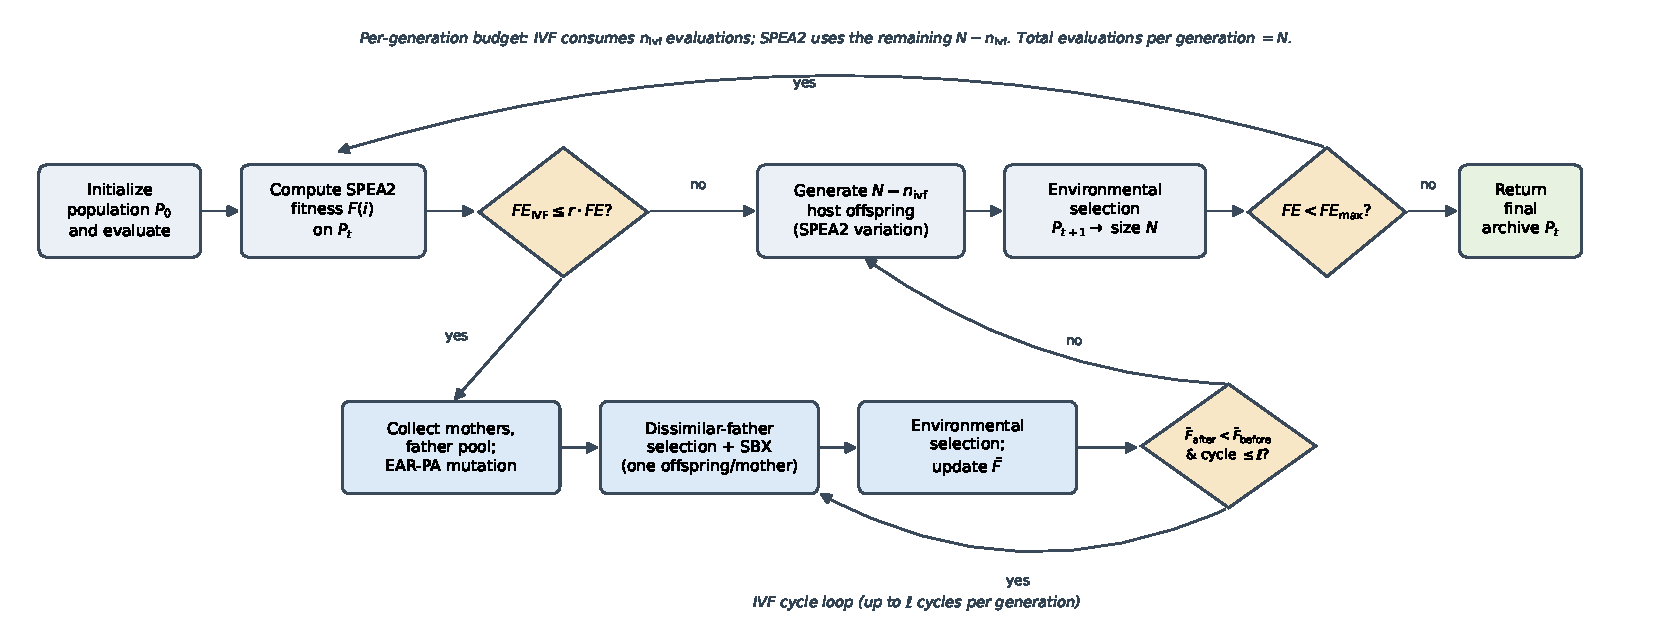
\includegraphics[width=\textwidth]{../figures/flowchart.pdf}
	\caption{Operational flow of IVF/SPEA2 under a fixed per-generation evaluation budget. The flowchart highlights the conditional IVF trigger, the intra-generation collective cycling rule, and the remaining-budget hand-off to canonical SPEA2 variation.}\label{fig:flow}
\end{figure*}


The IVF control parameters are the execution rate $r$, collection size $c$, and maximum number of IVF cycles $\ell$. The default setting is $c=0.12$, $r=0.225$, and $\ell=2$, with EAR-PA parameters $m=0.3$ and $v=0.1$; the selection rationale is detailed in Section~\ref{subsec:sensitivity}.

\subsection{IVF operator used in this study}\label{subsec:ivf-operator}
IVF operators include Assisted Recombination (AR) and its exploratory AR variants: EAR-N, EAR-T, EAR-P, and EAR-PA \citep{camilo-junior2011, sampaio2017ivf, Sampaio2024}. We instantiate IVF/SPEA2 with \textbf{EAR-PA}, which mutates a fraction of mothers before recombination and therefore injects local perturbation while retaining search around high-quality regions.

In all experiments, EAR-PA applies polynomial mutation ($\eta_m=20$) to a fraction $m=0.3$ of mothers and perturbs a fraction $v=0.1$ of decision variables per mutated mother. In the canonical implementation, the mutated mothers are the lowest-ranked mothers within the selected mother set rather than a random subset. Within each activated generation, the IVF cycle proceeds as follows:
\begin{enumerate}
	\item \textbf{Collection.} Sort by SPEA2 fitness $F(i)$ and set $n_p=\max(\operatorname{round}(cN),M+1)$. The top-$n_p$ individuals form the mother set. The father pool is the top $\operatorname{round}(N/2)$ by fitness. For each mother, Euclidean distances are computed on the raw objective vectors without additional normalization, the top-$K$ most distant non-self candidates are identified ($K=\min(3,|\text{pool}|)$), and the final father is chosen by binary tournament on fitness.
	\item \textbf{Recombination.} Mutate the lowest-ranked $\operatorname{round}(m n_p)$ mothers within the mother set, perturbing $\operatorname{round}(vD)$ randomly chosen variables per selected mother. Then recombine each mother with its assigned father using Simulated Binary Crossover (SBX) with $p_c=1$ and $\eta_c=20$ and evaluate one offspring per mother.
	\item \textbf{Selection and cycling.} Merge offspring with the current population and apply environmental selection to restore size $N$. Start a new IVF cycle only if mean SPEA2 fitness improves, i.e., $\bar{F}_{\text{after}} < \bar{F}_{\text{before}}$.
	\item \textbf{Budget adjustment.} If IVF consumes $n_{\text{ivf}}$ evaluations in the current generation, the host generates the remaining offspring quota with standard SPEA2 variation, i.e., binary tournament selection followed by PlatEMO's default genetic operator: SBX ($p_c=1$, $\eta_c=20$) and polynomial mutation ($p_m=1/D$, $\eta_m=20$). Under the production setting used in this paper ($N=100$, $c=0.12$), each IVF cycle consumes 12 evaluations, so the remaining host quota is always even and the combined generation uses exactly 100 evaluations.
\end{enumerate}

Self-recombination is prevented by excluding each mother from its father candidate set. The operator does not enforce explicit deduplication or one-to-one father matching; excessive concentration is handled indirectly by SPEA2's density term. In Algorithm~\ref{alg:ivf-spea2}, $P_t$ denotes the archive-sized working population returned by environmental selection, and $O_{\text{ivf}}$ and $O_{\text{host}}$ denote the temporary offspring buffers created within one generation. The pseudocode makes the activation trigger, the collective stopping criterion, the raw-objective father-distance rule, and the host-variation hand-off explicit.

\begin{algorithm}[!htbp]
	\caption{IVF/SPEA2 under a fixed function evaluation budget}\label{alg:ivf-spea2}
	\small
	\begin{algorithmic}[1]
		\Require Population size $N$, objective count $M$, decision dimension $D$, max evaluations $FE_{\max}$, execution rate $r$, collection size $c$, max IVF cycles $\ell$, mother mutation fraction $m$, variable mutation fraction $v$
		\State Initialize population $P_0$ with $N$ solutions; evaluate; $FE \gets N$; $FE_{\text{IVF}} \gets 0$; $t \gets 0$
		\State Set $P_t \gets P_0$
		\While{$FE < FE_{\max}$}
		\State Compute SPEA2 fitness on the current population $P_t$
		\State $n_{\text{ivf}} \gets 0$; $O_{\text{host}} \gets \varnothing$
		\If{$FE_{\text{IVF}} \le r \cdot FE$} \Comment{Activation trigger: cumulative IVF budget not exceeded}
		\State Sort $P_t$ by SPEA2 fitness $F(i)$ in ascending order
		\State Set $n_p \gets \max(\operatorname{round}(c\cdot N), M+1)$; Mothers $\gets$ top-$n_p$ individuals
		\State Father pool $\gets$ top-$\operatorname{round}(N/2)$ individuals by fitness
		\State Apply polynomial mutation ($\eta_m=20$) to the $\operatorname{round}(m \cdot n_p)$ lowest-ranked mothers, perturbing $\operatorname{round}(v \cdot D)$ randomly chosen variables each \Comment{EAR-PA}
		\For{$\text{cycle} = 1$ \textbf{to} $\ell$}
		\State $O_{\text{ivf}} \gets \varnothing$
		\If{$n_{\text{ivf}} + |$Mothers$| > N$} \textbf{break} \Comment{Per-generation budget}
		\EndIf
		\State $\bar{F}_{\text{before}} \gets$ mean fitness of current population
		\For{each mother $\mathbf{m}_i$ in Mothers} \Comment{Father chosen independently per mother}
		\State Compute Euclidean distances in raw objective space from $\mathbf{m}_i$ to all father-pool candidates (excluding self)
		\State Select top-$K$ ($K{=}\min(3,|\text{pool}|)$) most distant; binary tournament by fitness $\to$ father$_i$
		\State Cross $\mathbf{m}_i$ with father$_i$ via SBX ($\eta_c{=}20$, $p_c{=}1$); evaluate offspring and append to $O_{\text{ivf}}$
		\EndFor
		\State $FE \gets FE + |$Mothers$|$; $FE_{\text{IVF}} \gets FE_{\text{IVF}} + |$Mothers$|$; $n_{\text{ivf}} \gets n_{\text{ivf}} + |$Mothers$|$
		\State Set $P_t \gets \mathrm{EnvironmentalSelection}(P_t \cup O_{\text{ivf}}, N)$
		\State $\bar{F}_{\text{after}} \gets$ mean fitness of updated population
		\If{$\bar{F}_{\text{after}} < \bar{F}_{\text{before}}$} \Comment{Collective improvement}
		\State Update father pool from new population ranking
		\Else
		\State \textbf{break} \Comment{No collective improvement; terminate IVF}
		\EndIf
		\EndFor
		\EndIf
		\If{$n_{\text{ivf}} < N$}
		\State Generate the remaining offspring quota using binary tournament selection and standard SPEA2 variation from $P_t$; store in $O_{\text{host}}$; evaluate; update $FE$
		\State Set $P_{t+1} \gets \mathrm{EnvironmentalSelection}(P_t \cup O_{\text{host}}, N)$
		\Else
		\State Set $P_{t+1} \gets P_t$
		\EndIf
		\State Set $P_t \gets P_{t+1}$; $t \gets t+1$
		\EndWhile
		\State \Return Final population/archive approximation $P_t$
	\end{algorithmic}
\end{algorithm}


\subsection{Coupling Strategy and Function Evaluation Budget}\label{subsec:coupling}
IVF is invoked before canonical SPEA2 offspring generation and behaves as a budgeted auxiliary operator. In each generation, IVF may generate $n_{\text{ivf}}$ offspring ($0 \le n_{\text{ivf}} \le N$) under the activation condition $FE_{\text{IVF}} \le r\cdot FE$, where $FE_{\text{IVF}}$ is cumulative IVF usage and $FE$ is cumulative total evaluations. SPEA2 then generates $N-n_{\text{ivf}}$ offspring with its standard operators. If IVF is not activated or terminates early, $n_{\text{ivf}}=0$ and the generation is identical to canonical SPEA2.

\subsection{Computational Cost and Overhead}\label{subsec:cost}
A single canonical SPEA2 generation requires $\mathcal{O}(N^2 M)$ for pairwise dominance and strength computation, $\mathcal{O}(N^2 \log N)$ for $k$-nearest-neighbor density estimation, and $\mathcal{O}(N D)$ for variation operators, giving a per-generation baseline of $\mathcal{O}(N^2(M + \log N) + ND)$.

In one activated IVF generation, father assignment computes raw-objective distances from each of $n_p$ mothers to a father pool of size $\operatorname{round}(N/2)$, yielding $\mathcal{O}(n_p N M)$ per cycle, where $n_p=\max(\operatorname{round}(cN),M+1)$. With at most $\ell$ cycles, this contributes $\mathcal{O}(\ell\, n_p N M)$. Each cycle also invokes one environmental selection at $\mathcal{O}(N^2(M + \log N))$, adding up to $\ell$ such calls. The IVF overhead per activated generation is therefore $\mathcal{O}(\ell\, N^2(M + \log N))$, i.e., the same asymptotic class as a single SPEA2 generation, scaled by the constant $\ell$. Because IVF is not activated every generation, since the trigger $FE_{\text{IVF}} \le r \cdot FE$ becomes harder to satisfy as the run progresses, the amortized overhead is strictly smaller than $\ell$ times the baseline.

Evaluation overhead is also tightly controlled. In the reported production configuration ($N=100$, $c=0.12$, $\ell\le2$), IVF consumes either 12 or 24 evaluations in an activated generation and the remaining host quota is 88 or 76, so the per-generation total remains exactly $N=100$ evaluations. More generally, the comparison in this paper is evaluation-normalized rather than runtime-normalized: IVF/SPEA2 incurs additional wall-clock cost from the extra environmental-selection calls and father-distance calculations.


\subsection{Adaptations for SPEA2 Integration}\label{subsec:adaptation}
SPEA2 selection differs from dominance-plus-crowding hosts because fitness is jointly determined by dominance strength and density:
\[
	F(i) = R(i) + D(i),
\]
where
\[
	R(i) = \sum_{j \in P_t \cup \bar{P}_t,\; j \prec i} S(j)
\]
is the raw dominance component, and
\[
	D(i) = \frac{1}{\sigma_i^k + 2}
\]
is the density component based on the $k$-th nearest-neighbor distance.

To align IVF with this archive logic, IVF/SPEA2 uses the two host-specific adaptations detailed in Section~\ref{subsec:ivf-operator}: dissimilar-father selection, which increases crossover diversity while retaining fitness pressure; and collective cycle continuation, which conditions additional cycles on population-level fitness improvement ($\bar{F}_{\text{after}}<\bar{F}_{\text{before}}$) rather than on individual offspring quality.


\section{Experimental Setup}\label{sec:setup}

\subsection{Platform and Algorithms}\label{subsec:platform}
Experiments were conducted in MATLAB using the PlatEMO platform \citep{platemo} to compare IVF/SPEA2 with established and additional MOEAs: SPEA2 \citep{zitzler2001spea2}, the multiform host variant MFO-SPEA2 \citep{jiao2023multiform}, SPEA2 with shift-based density estimation (SPEA2+SDE) \citep{li2014shift}, NSGA-II \citep{deb2002fast}, NSGA-III \citep{deb2014nsga3}, MOEA/D \citep{zhang2007moead}, AGE-MOEA-II \citep{panichella2022agemoeaii}, and AR-MOEA \citep{tian2018armoea}. All algorithms used the default parameter settings shipped with the frozen PlatEMO snapshot (version 24.2.0.2923080) included in the public tagged release for this study \citep{zambrano2026ivfspea2repo}. This avoids instance-wise retuning and keeps the comparison at the level of published default configurations.

The baseline set spans complementary MOEA families relevant to the host-coupling question: host-centered SPEA2 variants (SPEA2, MFO-SPEA2, SPEA2+SDE), canonical Pareto/decomposition methods (NSGA-II, NSGA-III, MOEA/D), and modern adaptive geometry/reference approaches (AGE-MOEA-II, AR-MOEA). The last group is included because it is often competitive when front geometry is irregular or when explicit reference adaptation is advantageous, even though these methods do not implement a memetic intensification module.\footnote{AGE-MOEA-II and AR-MOEA results were obtained from dedicated benchmark runs covering all 51 instances with 60 runs each under the same population size and evaluation budget as the other algorithms.}

IVF/SPEA2 uses the EAR-PA operator defined in Section~\ref{subsec:ivf-operator}, with the default parameterization obtained through the tuning pipeline in Section~\ref{subsec:sensitivity}. Table~\ref{tab:params} lists all experimental settings.

\begin{table*}[!htbp]
	\caption{Parameter settings used in the experiments (PlatEMO version 24.2.0.2923080). Shared settings are listed in the first block. All shared settings correspond to the PlatEMO default values for the respective implementations. Algorithms marked ``(shared settings only)'' have no additional tuneable parameters beyond those listed in the shared block. For NSGA-III and MOEA/D, PlatEMO synchronizes the population size with the number of Das--Dennis reference points or weight vectors, giving $N=100$ for $M=2$ and $N=91$ for $M=3$. For SPEA2 and SPEA2+SDE, the density pool size is $|P|=2N$ during environmental selection.}\label{tab:params}
	\centering
	\small
	\renewcommand{\arraystretch}{1.05}
	\begin{tabularx}{\textwidth}{@{} l X X @{}}
		\toprule
		Algorithm          & Parameter                                      & Value                                                           \\
		\midrule
		All algorithms     & Population size $N$ (fixed-population cases)   & 100                                                             \\
		                   & Evaluation budget $FE_{\max}$                  & 100{,}000                                                       \\
		                   & Independent runs                               & 60                                                              \\
		                   & Mating selection                               & Binary tournament (size 2)                                      \\
		                   & Crossover (SBX): $p_c,\eta_c$                  & $1,20$                                                          \\
		                   & Mutation (polynomial): $p_m,\eta_m$            & $1/D,20$                                                        \\
		\midrule
		SPEA2              & Archive size $\bar{N}$                         & $N$                                                             \\
		                   & Density: $k$-NN                                & $k=\lfloor\sqrt{|P|}\rfloor$                                    \\
		\midrule
		SPEA2+SDE          & Archive size $\bar{N}$                         & $N$                                                             \\
		                   & Density estimation                             & Shift-based (SDE)                                               \\
		                   & Density: $k$-NN                                & $k=\lfloor\sqrt{|P|}\rfloor$                                    \\
		\midrule
		NSGA-II            & Additional algorithm parameters                & (shared settings only)                                          \\
		\midrule
		NSGA-III           & Reference points                               & Das--Dennis \citep{das1998normal}                               \\
		                   & Population size $N$                            & 100 ($M=2$); 91 ($M=3$)                                         \\
		\midrule
		MOEA/D             & Aggregation type                               & \texttt{type}$=1$ (PBI, $\theta{=}5$)                           \\
		                   & Weight vectors                                 & Das--Dennis                                                     \\
		                   & Neighborhood $T$                               & $\lceil N/10 \rceil$ (10 for both $M=2$ and $M=3$)              \\
		                   & Population size $N$                            & 100 ($M=2$); 91 ($M=3$)                                         \\
		\midrule
		MFO-SPEA2          & Additional algorithm parameters                & (shared settings only)                                          \\
		\midrule
		AGE-MOEA-II        & Additional algorithm parameters                & (shared settings only)                                          \\
		\midrule
		AR-MOEA            & Additional algorithm parameters                & (shared settings only)                                          \\
		\midrule
		\textbf{IVF/SPEA2} & Collection rate $c$                            & 0.12                                                            \\
		                   & IVF trigger ratio $r$                          & 0.225                                                           \\
		                   & Max cycles $\ell$                              & 2                                                               \\
		                   & Mother mutation fraction $m$                   & 0.3                                                             \\
		                   & Variable mutation fraction $v$                 & 0.1                                                             \\
		                   & Offspring per crossover $N_{\text{offspring}}$ & 1                                                               \\
		                   & Genetic-manipulation profile                   & EAR-PA                                                          \\
		                   & Father selection                               & Dissimilar: top-3 by raw-objective distance, fitness tournament \\
		                   & Father pool                                    & Top $\operatorname{round}(N/2)$ by fitness                      \\
		                   & Cycle continuation                             & Collective: $\bar{F}_\text{after} < \bar{F}_\text{before}$      \\
		                   & Archive size $\bar{N}$                         & $N$                                                             \\
		\botrule
	\end{tabularx}
\end{table*}


\subsection{Benchmark Suites}\label{subsec:benchmarks}
The evaluation uses benchmark suites chosen to cover complementary front geometries and landscape properties:
\begin{itemize}
	\item \textbf{ZDT} \citep{zitzler2000comparison} offers bi-objective problems with diverse Pareto front geometries (convex, concave, disconnected).
	\item \textbf{DTLZ} \citep{deb2005scalable} extends evaluation to scalable objective counts and increasing dimensionality.
	\item \textbf{WFG} \citep{huband2006review} introduces transformations yielding complex geometries with characteristics such as non-separability, multimodality, and asymmetry.
	\item \textbf{MaF} \citep{cheng2017benchmark} provides scalable multi-objective problems with diverse front characteristics; in this study we use the tri-objective ($M=3$) configurations to test IVF/SPEA2 under challenging front geometries.
	\item \textbf{RWMOP} (Real-World Multi-Objective Problems) \citep{kumar2021benchmark} offers constrained engineering optimization problems with realistic objective interactions and feasibility landscapes. In this study, we use three RWMOP instances (RWMOP9, RWMOP21, and RWMOP8) to assess IVF/SPEA2 beyond synthetic suites.
\end{itemize}

\subsection{Engineering Problem Selection Protocol}\label{subsec:engineering-selection}
To limit selection bias, engineering problems were chosen from the PlatEMO RWMOP collection (RWMOP1--RWMOP50) using a lock-before-results protocol. Inclusion required $M\in\{2,3\}$, the same evaluation budget as the synthetic experiments, feasible non-dominated solutions for IVF/SPEA2, and adequate metric availability (IGD and HV) across baselines.

The protocol had two stages:
\begin{enumerate}
	\item \emph{Feasibility probe}: IVF/SPEA2 was run once per candidate to verify feasible non-dominated solutions.
	\item \emph{Screening phase}: the full baseline set was run on a pre-frozen shortlist of six candidates (RWMOP8, RWMOP13, RWMOP20, RWMOP21, RWMOP24, RWMOP29) and evaluated by common-run coverage ($n=60$ target), feasible-run rate, and metric availability. RWMOP9 was retained separately as a pre-specified continuity benchmark from the earlier manuscript track.
\end{enumerate}

Screening outcomes varied across candidates:
\begin{itemize}
	\item RWMOP21: balanced profile (3/2/3 IGD wins/ties/losses, mirrored on HV);
	\item RWMOP8: adverse profile for IVF/SPEA2 (0/3/5);
	\item RWMOP20, RWMOP13, RWMOP24, RWMOP29: non-discriminative, with 0/8/0 pairwise signs and frequent missing metrics due to feasibility failures.
\end{itemize}

Three instances satisfied all inclusion criteria: RWMOP21 ($M=2$), RWMOP8 ($M=3$), and RWMOP9 ($M=2$, continuity benchmark). The final set deliberately includes an unfavorable case for IVF/SPEA2 (RWMOP8) to limit positive-selection bias and covers both objective-count settings.

\subsection{Performance Metric}\label{subsec:metric}
Performance was assessed primarily with Inverted Generational Distance (IGD), which measures both convergence and distribution by averaging distances from a reference Pareto set to the obtained approximation set. Lower IGD values indicate better approximation quality.

IGD was chosen as the primary indicator because it supports consistent per-instance comparisons across heterogeneous benchmark suites under fixed evaluation budgets. To avoid over-interpreting a single statistic, we report medians and interquartile ranges (IQR), complement significance tests with effect sizes ($A_{12}$), and discuss cases where practical degradation and statistical significance diverge. The role of HV as a secondary indicator is detailed in Section~\ref{subsec:stats}.

\subsection{Reference Sets for IGD and HV}\label{subsec:reference-sets}
For synthetic problems, IGD and HV are taken from PlatEMO's built-in metric outputs. In the frozen code snapshot used for this study, each problem instance constructs a problem-specific optimum/reference set as \texttt{Problem.GetOptimum(10000)} before optimization. IGD is then computed as the mean distance from this 10{,}000-point reference front sample to the final nondominated approximation, and HV uses the same problem-specific optimum set to determine the normalization bounds in PlatEMO's standard HV implementation, after which the reference point is the all-ones vector in normalized objective space \citep{platemo, zambrano2026ivfspea2repo}.

For engineering problems, built-in references are unsuitable or incomplete for robust comparison, so both metrics are recomputed offline from the final populations under common-run matching. IGD uses the empirical nondominated union of all feasible points across algorithms and selected runs for each problem, whereas HV uses each problem's \texttt{GetOptimum(10000)} output as the problem-specific reference set that determines the normalization bounds for the same PlatEMO HV routine. This recomputation is essential for RWMOP9, whose built-in optimum degenerates to a single point for IGD purposes.

\subsection{Statistical Analysis and Protocol}\label{subsec:stats}

\textbf{Primary endpoint.} IGD is the pre-specified primary performance indicator. All primary inferential claims, including multiplicity-corrected win/loss/tie summaries, are based on IGD. HV is treated as a secondary indicator: when reported, it serves as complementary instance-level evidence and is not used to confirm the primary claim.

\textbf{Pairwise significance testing.} For each benchmark instance, we compare the 60 IGD values of IVF/SPEA2 against each baseline using the Wilcoxon rank-sum test \citep{wilcoxon1945} (two-sided, $\alpha=0.05$). A nonparametric test is appropriate because IGD distributions can be skewed and may violate normality assumptions. Unless stated otherwise, table symbols ($+$, $-$, $\approx$) correspond to these unadjusted pairwise tests.

\textbf{Multiplicity correction.} The primary claim, IVF/SPEA2 versus SPEA2 across instances, involves 28 simultaneous hypotheses for $M=2$ and 23 for $M=3$. To control the family-wise error rate, we apply the Holm--Bonferroni step-down procedure \citep{holm1979simple} separately for each objective count. Corrected counts are reported alongside unadjusted counts in Section~\ref{subsec:results-spea2}.

\textbf{Effect size.} To complement binary significance decisions with a measure of practical magnitude, we report the Vargha--Delaney $A_{12}$ statistic \citep{vargha2000critique} for every instance--baseline pair. $A_{12}$ estimates the probability that a randomly drawn IVF/SPEA2 run produces a smaller IGD than a randomly drawn baseline run. Values of $A_{12}=0.5$ indicate stochastic equality; values above 0.56, 0.64, and 0.71 correspond to small, medium, and large effects in favor of IVF/SPEA2, respectively, following the original thresholds \citep{vargha2000critique}. Effect-size heatmaps are reported in the Results section.

\textbf{Rationale for pairwise rather than omnibus testing.} When comparing $k>2$ algorithms across $n$ instances, tutorial treatments often use Friedman-family omnibus tests followed by post-hoc procedures such as Nemenyi \citep{derrac2011practical}. Here, the primary scientific question is whether IVF intensification improves its \emph{own host} (SPEA2), not which algorithm attains the best overall rank. The remaining seven baselines serve as contextual comparators rather than as co-equal hypotheses in a single ranking. We therefore use pairwise Wilcoxon tests with Holm--Bonferroni correction for the primary IVF/SPEA2-vs.-SPEA2 comparison, and report unadjusted pairwise tests against the remaining baselines as exploratory evidence. This keeps multiplicity control aligned with the central question without inflating the hypothesis space.

\textbf{Replication and run protocol.} Each benchmark configuration was executed 60 times for IVF/SPEA2 and for each of the eight baseline algorithms. The choice of $n=60$ reflects a deliberately conservative run budget for stochastic-optimization experimentation, for which run-count selection materially affects estimate reliability \citep{eftimov2025adaptive}, and it stabilizes Wilcoxon testing together with median and IQR estimation. The same 60-run protocol applies to both the synthetic suites and the engineering RWMOP suite, with the latter using robust common-run matching and empirical Pareto-front recomputation for IGD and HV.

After cohort filtering, the primary IVF/SPEA2-vs.-SPEA2 comparison retains complete 60-vs.-60 coverage on all 51 synthetic instances; all claim tables are computed from this filtered cohort only.

\textbf{HV coverage.} HV is available for all nine algorithms across all 51 synthetic instances, and is reported in Appendix~\ref{app:tables} and in the aggregate claim summary (Table~\ref{tab:claims_summary}).

\subsection{Parameter Tuning Pipeline}\label{subsec:sensitivity}
To identify a robust default configuration for IVF/SPEA2's five key parameters ($c$, $r$, $\ell$, $m$, $v$), we conducted a three-phase tuning pipeline on a representative 12-problem subset spanning bi- and tri-objective settings.\footnote{Tuning subset: ZDT1, ZDT6, WFG4, WFG9 ($M=2$); DTLZ1, DTLZ2, DTLZ4, DTLZ7, WFG2, WFG5, MaF1, MaF5 ($M=3$).} Each configuration was evaluated over 30 independent runs ($N=100$, $\mathrm{FE}_{\max}=50{,}000$) using both IGD and HV.

\textbf{Phase~A (Execution/Collection Grid).} The first phase isolates the execution and collection parameters under pure AR ($m=0$, $v=0$). A grid of $r \in \{0.05, 0.10, 0.15, 0.20\}$, $c \in \{0.07, 0.11, 0.16, 0.21\}$, and $\ell \in \{2, 3, 4\}$ was evaluated (48 configurations, 17{,}280 total runs). Configuration A43 ($r=0.20$, $c=0.16$, $\ell=2$) attained the best mean combined rank across the 12-problem tuning subset. Fig.~\ref{fig:sensitivity}(a) shows the Phase~A landscape for the Cycles$\,{=}\,2$ slice and indicates a broad high-ranking region rather than a single isolated cell.

\textbf{Phase~B (Operator Comparison).} The second phase evaluates five operator profiles at the Phase~A center ($r=0.20$, $c=0.16$, $\ell=2$): (B01)~AR ($m=0$, $v=0$); (B02)~EAR-PA ($m=0.3$, $v=0.1$); (B03)~EAR-P ($m=0.5$, $v=0.2$); (B04)~EAR-T ($m=0.7$, $v=0.3$); (B05)~EAR-N ($m=0.5$, $v=0.2$, random re-initialization). As shown in Fig.~\ref{fig:sensitivity}(b), EAR-PA (B02) achieved the best mean combined rank, suggesting that polynomial mutation on 30\% of mothers improves offspring quality without excessive disruption.

\textbf{Phase~C (Local Refinement).} The third phase performs a local grid search around the Phase~A/B center, varying $r \in \{0.175, 0.200, 0.225\}$, $c \in \{0.12, 0.16, 0.21\}$, and four operator profiles (AR, EAR-PA, EAR-P, EAR-N), totaling 36 configurations. Configuration C26 ($r=0.225$, $c=0.12$, $\ell=2$, $m=0.3$, $v=0.1$) achieved the best mean combined rank and was selected as the promoted configuration; Fig.~\ref{fig:sensitivity}(c) displays the corresponding EAR-PA slice.

\textbf{Validation.} Head-to-head comparison using Mann--Whitney $U$ tests with Holm--Bonferroni correction ($\alpha=0.05$) across the 12-problem tuning subset shows no corrected IGD difference between C26 and A43 (0 wins, 12 ties, 0 losses). Both C26 and A43 achieve 4 corrected wins, 8 ties, and 0 losses against the original pre-tuning baseline ($c=0.11$, $r=0.10$, AR, $\ell=3$). C26 was promoted because it combines the activation/collection refinement from Phase~A with the operator improvement identified in Phases~B/C.

\begin{figure*}[t]
	\centering
	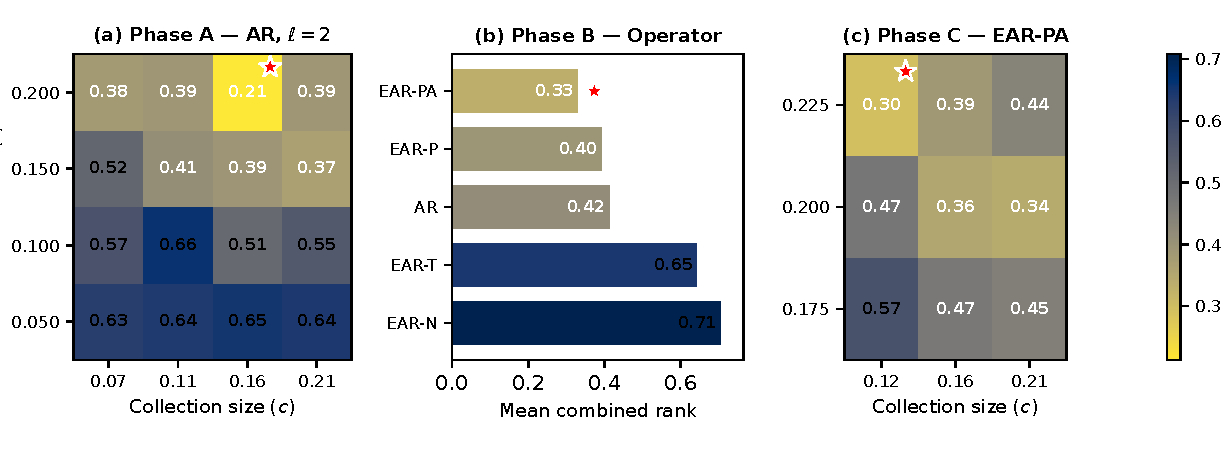
\includegraphics[width=\textwidth]{../figures/tuning_heatmap_combined.pdf}
	\caption{Tuning pipeline results derived from the actual parameter search on the 12-problem tuning subset (30 runs each). Color encodes mean combined rank across the subset (lower is better, darker shading); cell/bar values are annotated. (a)~Phase~A broad search ($4 \times 4$ grid over $r$ and $c$, Cycles$\,{=}\,2$, pure AR): the starred cell marks configuration A43 ($r=0.20$, $c=0.16$). (b)~Phase~B operator comparison (5 profiles at the Phase~A center): EAR-PA ($m=0.3$, $v=0.1$) achieves the best rank. (c)~Phase~C local refinement ($3 \times 3$ grid over $r$ and $c$, EAR-PA): the starred cell marks the promoted configuration C26 ($r=0.225$, $c=0.12$), selected as the default for all subsequent experiments.}
	\label{fig:sensitivity}
\end{figure*}

\textbf{Separation of tuning and confirmatory evaluation.} The tuning pipeline (Phases~A--C) was conducted exclusively on the 12-problem tuning subset using a reduced budget ($\mathrm{FE}_{\max}=50{,}000$, 30 runs). The main evaluation (Section~\ref{sec:results}) applies the promoted configuration C26 to the full 51-instance benchmark set under the production budget ($\mathrm{FE}_{\max}=100{,}000$, 60 runs), which includes 39 instances not seen during tuning. The 12 tuning instances reappear in the main evaluation under a different budget and sample size, which provides only partial independence; results on those instances should therefore be interpreted with that caveat. The main comparison remains \emph{defaults versus defaults}: C26 is frozen as the IVF/SPEA2 default, and no per-experiment retuning is applied to any algorithm during the confirmatory study. Under this symmetric protocol, the 39 out-of-sample instances provide the primary evidence for generalization.

\subsection{Threats to validity}\label{subsec:validity}
\textbf{Internal validity.} IVF/SPEA2 uses the parameterization selected by the tuning pipeline on a representative subset of 12 problems (Section~\ref{subsec:sensitivity}). Different parameterizations could change the observed gains, and the tuning set does not cover all 51 benchmark instances. All configurations use 60 independent runs with nonparametric tests (Section~\ref{subsec:stats}).

\textbf{Construct validity.} Performance is measured primarily with IGD, which captures both convergence and distribution relative to a reference set. Although IGD is widely used in multi-objective optimization, conclusions can change under alternative indicators such as hypervolume, especially on instances with irregular fronts or high dispersion. We mitigate this risk through IQR reporting, $A_{12}$ effect-size analysis, and a secondary HV analysis with complete cross-algorithm coverage (Section~\ref{subsec:stats}). HV-based counts (Table~\ref{tab:claims_summary}) generally support the IGD findings for the primary IVF/SPEA2-versus-SPEA2 comparison, although several instances show indicator disagreement discussed in Sections~\ref{subsec:results-spea2} and~\ref{subsec:engineering}.

\textbf{Conclusion validity.} Holm--Bonferroni correction (Section~\ref{subsec:stats}) is applied to control family-wise error for the primary comparison. The resulting reduction in significant wins confirms that part of the raw advantage is small and should be interpreted conservatively.

\textbf{External validity.} The evaluation focuses on synthetic benchmark suites (ZDT, DTLZ, WFG, MaF) and three constrained engineering problems (RWMOP9, RWMOP21, RWMOP8). These benchmarks cover diverse front geometries, but they do not exhaust the range of real-world objective interactions. The current scope is limited to $M=2$ and $M=3$; conclusions should therefore not be extrapolated to higher-dimensional settings without additional evidence. The engineering suite extends the assessment beyond a single case, but broader validation on additional real-world domains and higher-dimensional objectives would strengthen external validity. Implementing IVF/SPEA2 within PlatEMO improves reproducibility, although framework-level choices, including IVF operator details, can still influence outcomes.%


\section{Results}\label{sec:results}

This section reports the empirical performance of IVF/SPEA2 under its default configuration (Table~\ref{tab:params}). The main confirmatory claim is the pairwise comparison against the canonical host, SPEA2; the remaining analyses provide mechanism-level interpretation, broader competitive positioning, and transferability evidence.

To make the evidence trail explicit, Table~\ref{tab:claims_summary} consolidates the main claim-relevant counts before the detailed tables and figures. Unless noted otherwise, entries are wins/losses/ties from IVF/SPEA2's perspective. We first report the host comparison against SPEA2, then broader synthetic positioning and engineering transferability, and finally the supportive ablation evidence for the current implementation.

\begin{table}[t]
	\caption{Claim-oriented summary of the main quantitative evidence (IVF/SPEA2 vs.\ SPEA2, synthetic instances only). Based on 28 bi-objective and 23 tri-objective synthetic instances (51 total). Counts are wins/losses/ties from IVF/SPEA2's perspective. OOS denotes out-of-sample instances not used during tuning: 24 for $M{=}2$ and 15 for $M{=}3$, totaling 39. The ``Holm, OOS'' row applies Holm--Bonferroni correction across all instances within each $M$ group and then filters to OOS, providing the most conservative evidence layer. Per-instance table symbols are based on unadjusted tests; Holm rows apply family-wise correction across all instances within each $M$ group. IGD is the primary indicator; HV is reported as secondary confirmation.}
	\label{tab:claims_summary}
	\centering
	\scriptsize
	\begin{tabular}{lcc}
		\toprule
		Evidence block                         & $M=2$  & $M=3$                 \\
		\midrule
		\multicolumn{3}{l}{\textit{Primary indicator (IGD, lower is better)}}   \\
		IVF/SPEA2 vs.\ SPEA2 (unadjusted)      & 23/3/2 & 18/1/4                \\
		IVF/SPEA2 vs.\ SPEA2 (unadjusted, OOS) & 20/2/2 & 13/0/2                \\
		IVF/SPEA2 vs.\ SPEA2 (Holm)            & 22/3/3 & 15/1/7                \\
		IVF/SPEA2 vs.\ SPEA2 (Holm, OOS)       & 19/2/3 & 12/0/3                \\
		\midrule
		\multicolumn{3}{l}{\textit{Secondary indicator (HV, higher is better)}} \\
		IVF/SPEA2 vs.\ SPEA2 (unadjusted)      & 23/3/2 & 17/1/5                \\
		IVF/SPEA2 vs.\ SPEA2 (unadjusted, OOS) & 20/2/2 & 11/0/4                \\
		IVF/SPEA2 vs.\ SPEA2 (Holm)            & 22/3/3 & 17/1/5                \\
		IVF/SPEA2 vs.\ SPEA2 (Holm, OOS)       & 19/2/3 & 11/0/4                \\
		\botrule
	\end{tabular}
\end{table}

\subsection{Primary Comparison: IVF/SPEA2 vs.\ SPEA2}\label{subsec:results-spea2}
We first compare IVF/SPEA2 directly with canonical SPEA2. Unless noted otherwise, per-instance signs are based on unadjusted Wilcoxon rank-sum tests ($p < 0.05$) applied to IGD values.

Because parameter selection used the 12-problem tuning subset, the most decision-relevant evidence is the 39-instance out-of-sample partition. On those unseen synthetic instances, IVF/SPEA2 records unadjusted IGD counts of 20/2/2 for $M=2$ and 13/0/2 for $M=3$. Applying Holm--Bonferroni correction across all instances within each objective-count group and then filtering to the out-of-sample cases yields the most conservative evidence layer: 19/2/3 for $M=2$ and 12/0/3 for $M=3$. The main gain pattern therefore persists outside the subset used for parameter selection.

Over the full synthetic suite, IVF/SPEA2 achieves significant IGD improvements in 23 of 28 bi-objective instances with 3 losses, and 18 of 23 tri-objective instances with 1 loss. After Holm--Bonferroni correction, the counts become 22/3/3 for $M=2$ and 15/1/7 for $M=3$. Table~\ref{tab:claims_summary} consolidates these counts alongside the secondary hypervolume indicator. Hypervolume broadly supports the same pattern, with its losses concentrated on disconnected or irregular front geometries.

Per-instance median IGD shifts provide a complementary practical view of the host comparison. Fig.~\ref{fig:effect-magnitude} plots the percentage improvement of IVF/SPEA2 over SPEA2 on every synthetic instance and distinguishes the 39 out-of-sample cases from the 12 instances used during tuning. The purpose of this figure is not to add another significance layer, but to show where the host-level gain is concentrated and whether the observed advantage is confined to tuned cases. The pattern is broad but mostly moderate: the median shift is positive on 24 of 28 bi-objective instances and 21 of 23 tri-objective instances, with overall median improvements of +1.25\% and +0.99\%, respectively. The strongest positive excursion occurs on WFG1 ($M=2$, +24.1\%), whereas the negative bars are concentrated on disconnected or irregular cases, especially WFG2, WFG3, and WFG9 at $M=2$ and WFG2 at $M=3$. Positive bars also remain predominant in the out-of-sample partition, which is the key generalization target of the study. Per-instance tables are provided in Appendix~\ref{app:tables}.

\begin{figure*}[t]
	\centering
	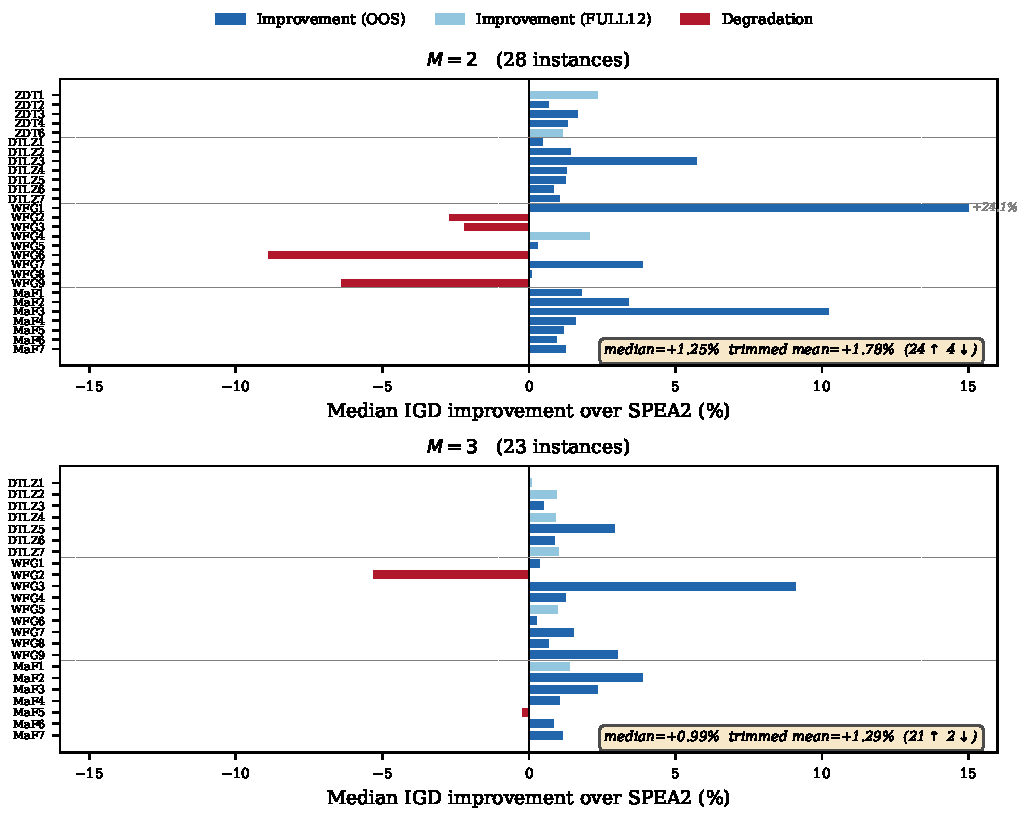
\includegraphics[width=0.84\textwidth]{../figures/effect_magnitude_igd.pdf}
	\caption{Per-instance median IGD improvement of IVF/SPEA2 over SPEA2 on all synthetic instances. Positive values favor IVF/SPEA2 because lower IGD is better; negative values indicate degradation. Dark blue bars denote out-of-sample instances not used during tuning, light blue bars denote the 12 tuning instances, and red bars denote negative median shifts. Values beyond $\pm 15\%$ are clipped for display and annotated with their true magnitude.}
	\label{fig:effect-magnitude}
\end{figure*}

Whereas Fig.~\ref{fig:effect-magnitude} localizes the median effect size instance by instance, Figs.~\ref{fig:boxplot-m2} and~\ref{fig:boxplot-m3} display the full IGD distributions for IVF/SPEA2 versus SPEA2 across all instances. The tight, well-separated boxes on many ZDT and DTLZ instances show that the wins are not outlier driven, whereas the wide spread on DTLZ4($M=3$) foreshadows the bimodal convergence regime discussed later.

\begin{figure*}[t]
	\centering
	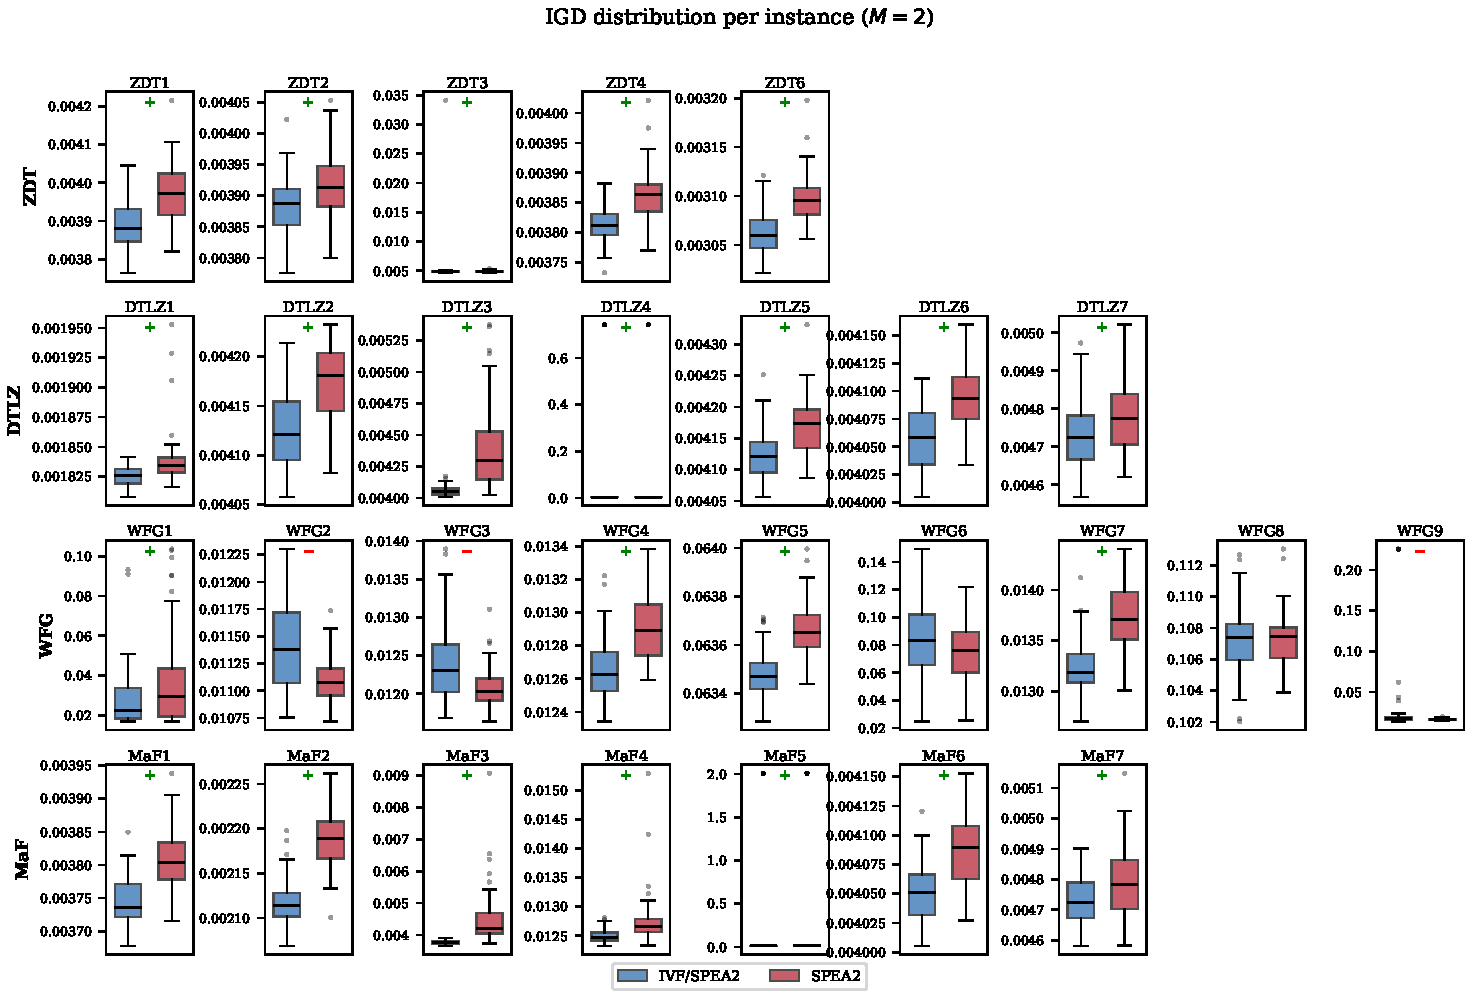
\includegraphics[width=\textwidth]{../figures/boxplot_igd_m2.pdf}
	\caption{IGD distributions for IVF/SPEA2 and SPEA2 on all bi-objective instances ($M=2$), grouped by benchmark suite. Each box spans the interquartile range over 60 independent runs, and whiskers extend to $1.5\times$IQR. The significance marks identify unadjusted Wilcoxon rank-sum outcomes from IVF/SPEA2's perspective. Lower IGD is better.}\label{fig:boxplot-m2}
\end{figure*}

\begin{figure*}[t]
	\centering
	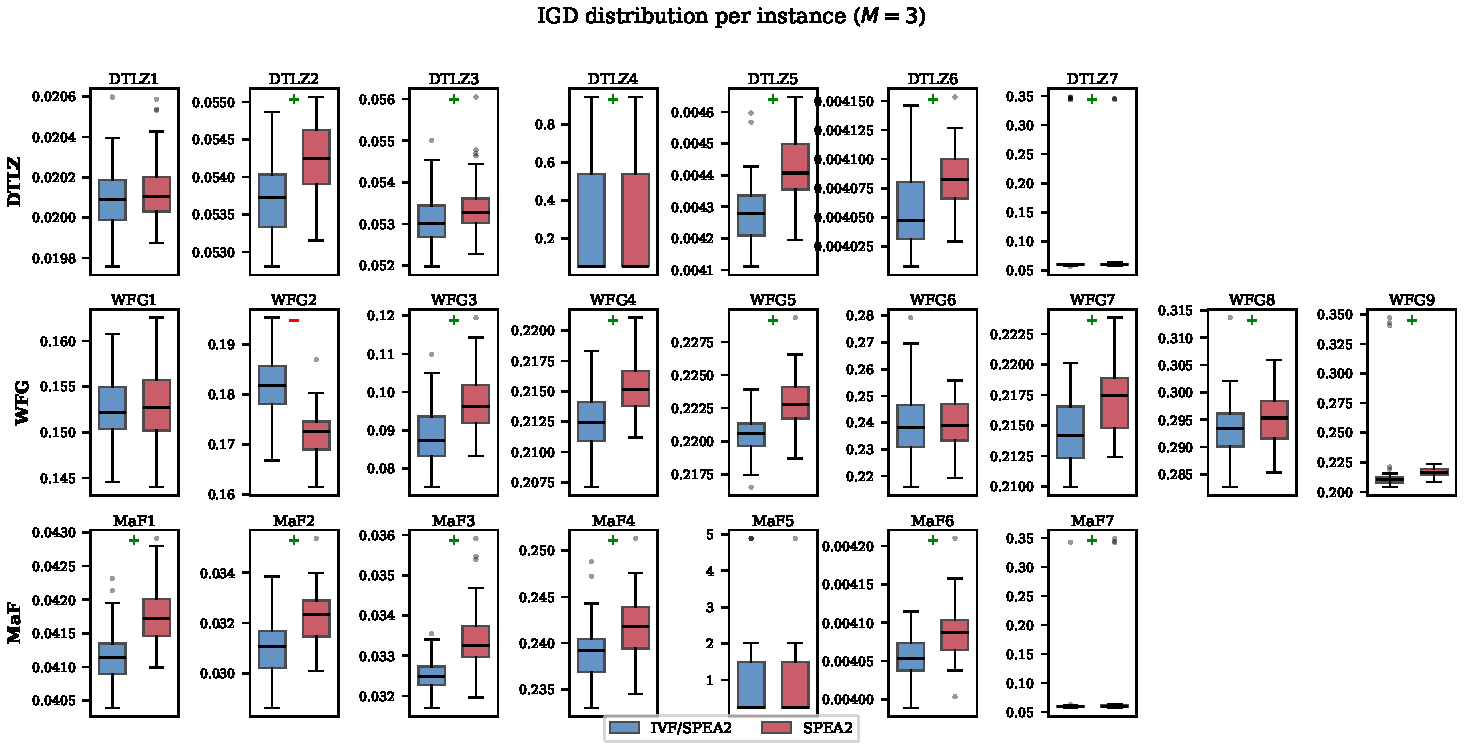
\includegraphics[width=\textwidth]{../figures/boxplot_igd_m3.pdf}
	\caption{IGD distributions for IVF/SPEA2 and SPEA2 on all tri-objective instances ($M=3$). The broad spread on DTLZ4 and the clear loss on WFG2 indicate that the hybrid is not uniformly beneficial, even when the median remains competitive on most instances.}\label{fig:boxplot-m3}
\end{figure*}

\subsection{Exploratory Positioning Against Additional Baselines}\label{subsec:results-detailed}
Exploratory multi-baseline results are reported in Supplementary Information~1; they are useful for regime interpretation but do not replace the primary IVF/SPEA2-versus-SPEA2 comparison. The suite-level pattern is nevertheless consistent with the host-specific claim. In the bi-objective setting, IVF/SPEA2 beats SPEA2 on all five ZDT instances and all seven DTLZ instances. On WFG, the record against SPEA2 is 4/3/2, with losses concentrated on WFG2, WFG3, and WFG9, all of which involve disconnected or irregular front structures. On MaF, the record is 7/0/0. In the tri-objective setting, the corresponding records against SPEA2 are 6/0/1 on DTLZ, 6/1/2 on WFG, and 6/0/1 on MaF. The dominant tri-objective loss remains WFG2, while DTLZ4 and MaF5 exhibit high dispersion rather than a uniformly poor median.

Exploratory average-rank analysis places IVF/SPEA2 second for $M=2$ (3.11) and first for $M=3$ (2.22) across the nine algorithms considered, but we treat those ranks only as contextual navigation because the confirmatory question in this paper is host improvement rather than global algorithm ordering.

Figs.~\ref{fig:a12-m2} and~\ref{fig:a12-m3} summarize the Vargha--Delaney $A_{12}$ effect sizes against all baselines. The heatmaps show near-uniform advantages over SPEA2+SDE and NSGA-II, whereas AGE-MOEA-II emerges as the strongest synthetic-suite competitor, particularly at $M=3$. Adverse cells again concentrate on disconnected or irregular geometries, especially WFG2 and, more weakly, WFG6 and MaF5.

\begin{figure*}[t]
	\centering
	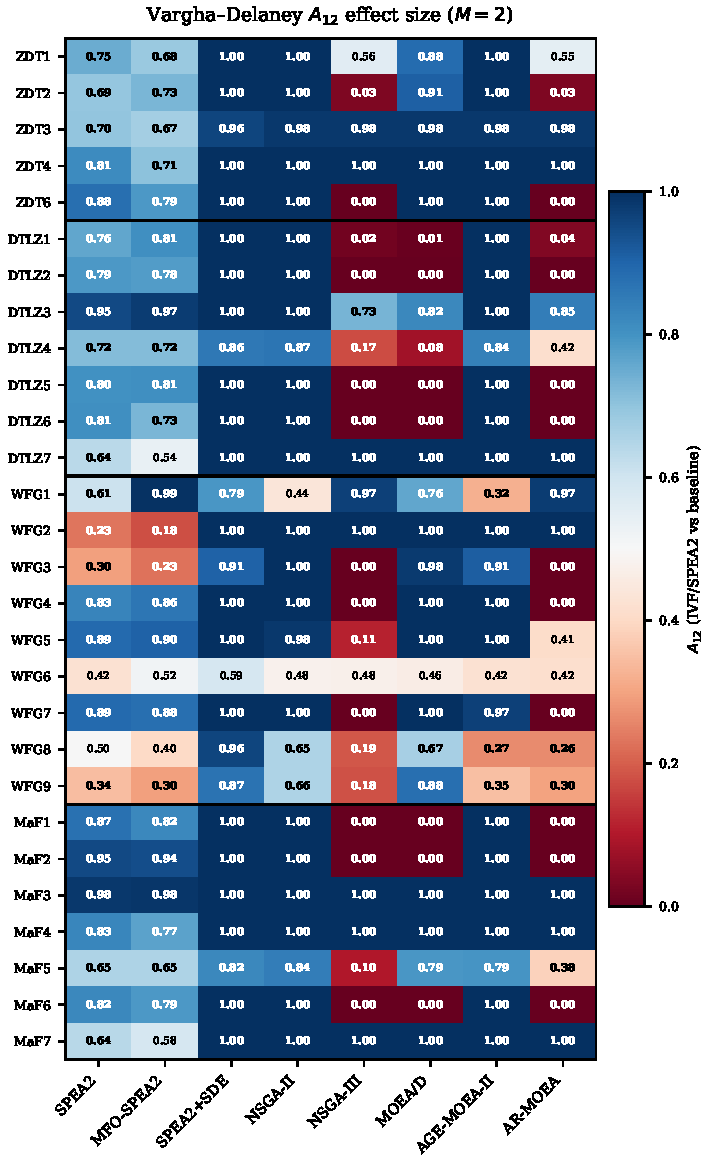
\includegraphics[width=0.82\textwidth]{../figures/heatmap_a12_M2.pdf}
	\caption{Vargha--Delaney $A_{12}$ effect size for IVF/SPEA2 versus each baseline on bi-objective instances ($M=2$). Values above 0.5 indicate an IVF/SPEA2 advantage and values below 0.5 indicate a baseline advantage. Bold values denote unadjusted Wilcoxon significance, and horizontal separators mark benchmark-suite boundaries.}\label{fig:a12-m2}
\end{figure*}

\begin{figure*}[t]
	\centering
	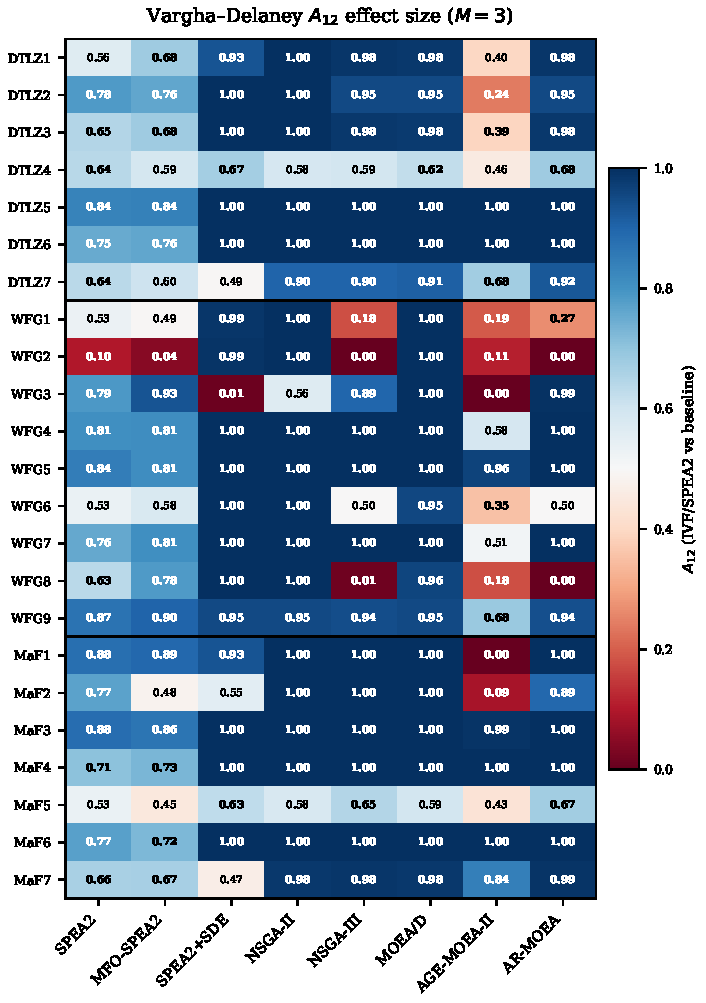
\includegraphics[width=0.82\textwidth]{../figures/heatmap_a12_M3.pdf}
	\caption{Vargha--Delaney $A_{12}$ effect size for IVF/SPEA2 versus each baseline on tri-objective instances ($M=3$). AGE-MOEA-II is the strongest competitor in several DTLZ and WFG cases, while WFG2 and MaF5 show the clearest adverse cells for IVF/SPEA2.}\label{fig:a12-m3}
\end{figure*}

\FloatBarrier
\subsection{Engineering Benchmarks: RWMOP Suite}\label{subsec:engineering}
To extend the evaluation beyond synthetic suites, we test IVF/SPEA2 on three constrained real-world RWMOP problems from PlatEMO: the bi-objective problems RWMOP9 and RWMOP21, and the tri-objective problem RWMOP8. Selection follows the pre-defined protocol in Section~\ref{subsec:engineering-selection}, which ensures meaningful common-run coverage under identical budgets. The three cases cover distinct design contexts: RWMOP9 is a four-bar plane-truss trade-off between structural mass and deflection, RWMOP21 models high-speed-train crash-energy management under safety constraints, and RWMOP8 is a car side-impact design problem with three objectives balancing weight, intrusion, and structural response.

Following the robust post-processing protocol, IGD is recomputed against the empirical nondominated reference front defined by the union of feasible points collected across algorithms and selected common runs. Hypervolume is recomputed with the same PlatEMO routine used in the synthetic study, using each problem's \texttt{GetOptimum(10000)} output to determine the normalization bounds. We use strict common-run matching with 60 runs per algorithm and $N=100$, $\mathrm{FE}_{\max}=100{,}000$. This engineering track is executed independently from the synthetic submission runs, with 60 dedicated runs per algorithm and problem.\footnote{Engineering-suite scripts and data paths are documented in the code repository (see Code Availability).} Not all algorithms produce valid metric values on every problem: on RWMOP8, SPEA2+SDE yields valid IGD/HV in only 18 of 60 runs because of low feasibility, and MOEA/D produces zero feasible runs, which excludes it from statistical comparison on that instance.

Table~\ref{tab:engineering} summarizes the pairwise signs against IVF/SPEA2 across the full baseline set. The pattern is strongly problem dependent. On RWMOP9, IVF/SPEA2 wins all pairwise IGD comparisons (8/0/0) and 5 of 8 HV comparisons (5/0/3). On RWMOP21, both IGD and HV are balanced (3/2/3), with clear wins and losses against different baselines. On RWMOP8, IVF/SPEA2 is unfavorable under both indicators, with counts of 1/1/5 for IGD and 1/1/5 for HV. MOEA/D is excluded from this instance because of zero valid runs. This shows that transferability is not uniform across engineering landscapes.

\begin{table}[t]
	\caption{Engineering suite under robust metric recomputation with common-run matching ($n=60$ target per algorithm). Entries are pairwise win/equal/loss counts from IVF/SPEA2's perspective against the eight baselines, using Wilcoxon rank-sum tests ($\alpha=0.05$).}\label{tab:engineering}
	\centering\small
	\begin{tabular}{lccc}
		\toprule
		Problem                   & $M$ & IGD ($+/\approx/-$) & HV ($+/\approx/-$) \\
		\midrule
		RWMOP9                    & 2   & 8/0/0               & 5/0/3              \\
		RWMOP21                   & 2   & 3/2/3               & 3/2/3              \\
		RWMOP8\textsuperscript{b} & 3   & 1/1/5               & 1/1/5              \\
		\botrule
	\end{tabular}
	\smallskip
	\noindent\textsuperscript{b} MOEA/D is excluded because it yields 0/60 valid runs; SPEA2+SDE contributes 18/60 valid runs only, which reduces statistical power for that pairwise comparison.
\end{table}

To show indicator magnitude and dispersion together with feasibility coverage, Fig.~\ref{fig:engineering-profiles} reports the median and IQR for each algorithm/problem under both IGD and HV, with explicit valid-run annotations ($n$). The figure confirms full coverage ($n=60$) on RWMOP9 and RWMOP21, and heterogeneous coverage on RWMOP8 (SPEA2+SDE: $n=18$; MOEA/D: $n=0$). Representative engineering fronts are provided in Supplementary Information~1.

\begin{figure*}[t]
	\centering
	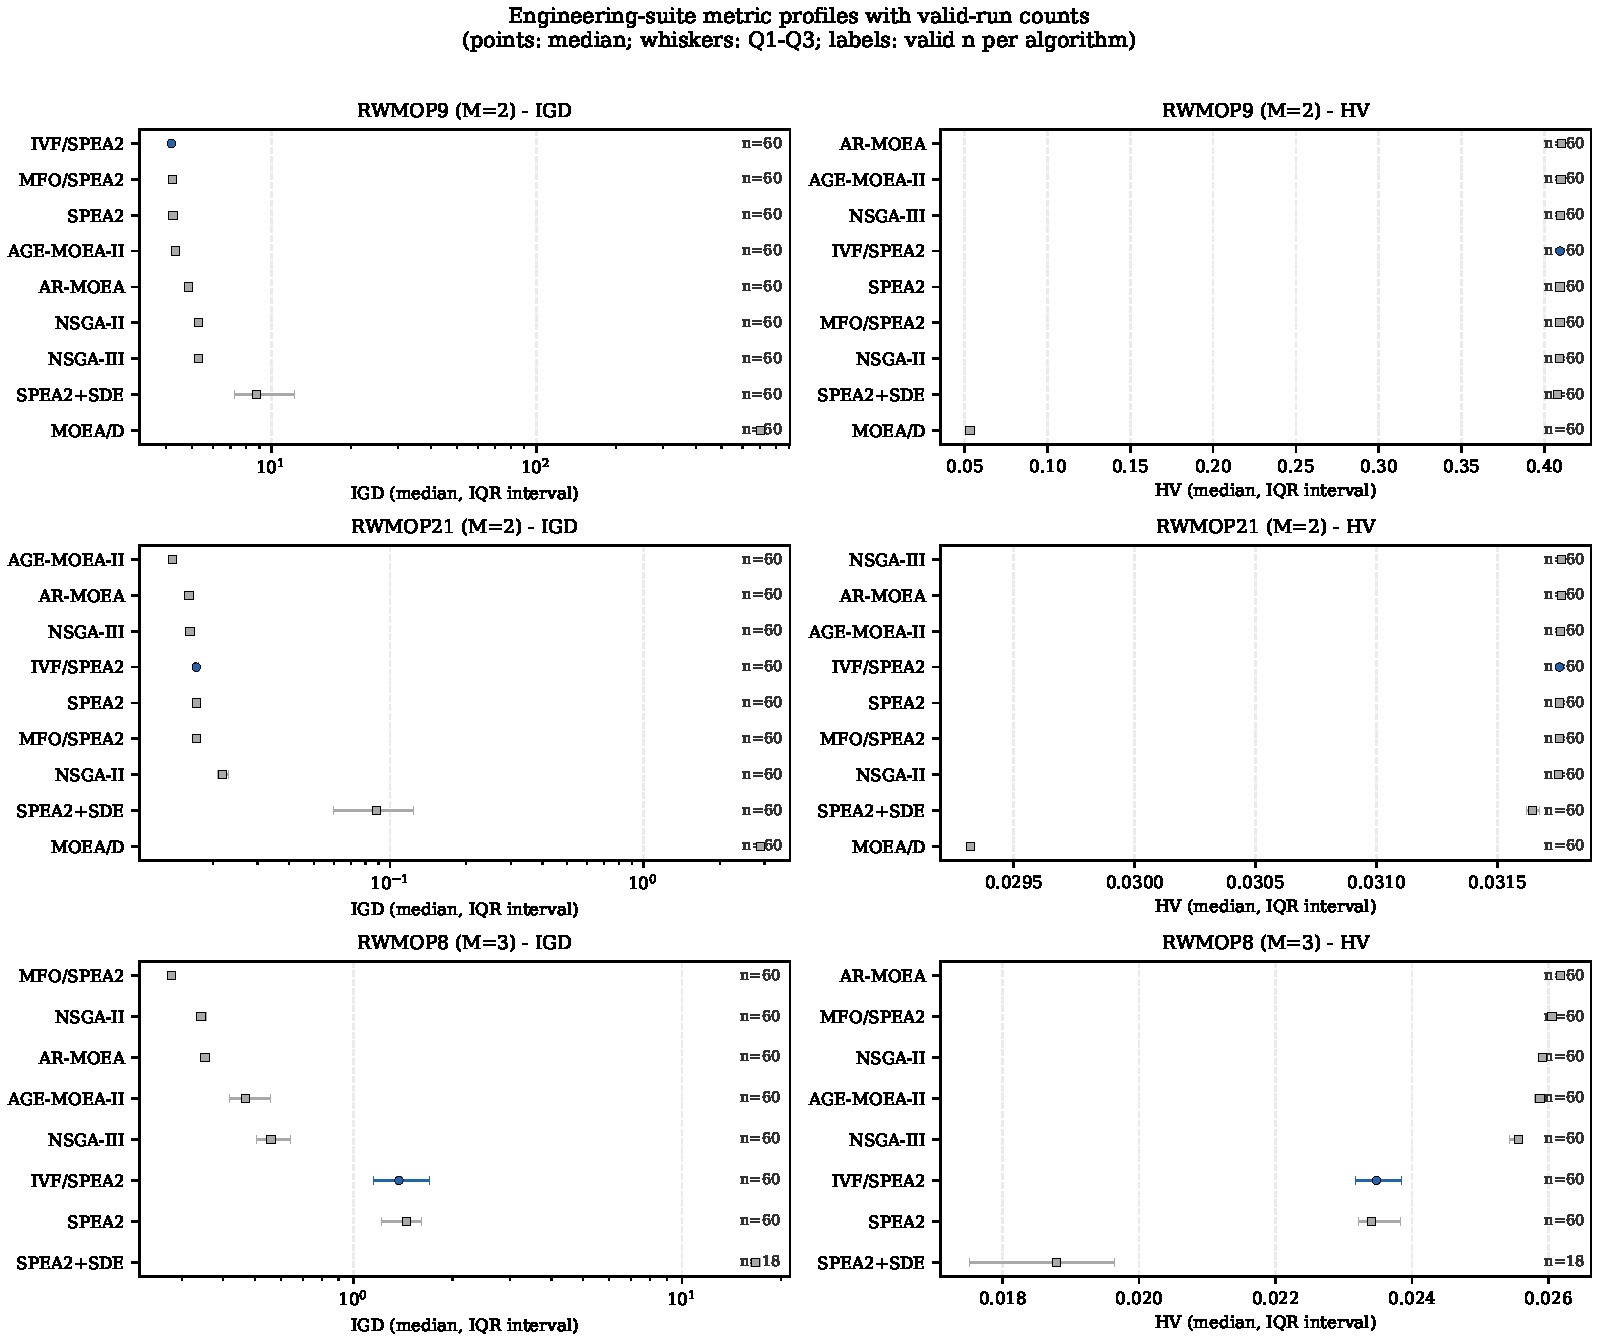
\includegraphics[width=0.94\textwidth]{../figures/engineering_metric_profiles.pdf}
	\caption{Engineering-suite metric profiles with explicit valid-run counts. Each point is the median over valid runs, whiskers show the interquartile interval ($Q_1$--$Q_3$), and labels indicate the valid sample size ($n$) per algorithm. Left column: IGD (log scale). Right column: HV. Coverage asymmetry is most visible on RWMOP8, where MOEA/D has no valid runs and SPEA2+SDE has partial coverage.}\label{fig:engineering-profiles}
\end{figure*}

The IGD--HV discordance on RWMOP9 illustrates a convergence--spread trade-off between indicators. IVF/SPEA2 dominates all baselines under IGD but loses three HV comparisons (against NSGA-III, AGE-MOEA-II, and AR-MOEA), which shows that algorithm ranking can change with the indicator even on the same instance. Taken together, the engineering evidence should therefore be read as a bounded transferability check rather than as broad practical validation.

\FloatBarrier
\subsection{Supportive Design Validation}\label{subsec:ablation}
This section tests whether dissimilar-father selection and collective cycle continuation independently contribute to performance, or whether they are best understood as implementation refinements of the host-specific coupling. Supportive ablation material is collected in Supplementary Information~1 because it does not underpin the paper's primary confirmatory claim. Three points matter for the main manuscript. First, on the 12-problem tuning subset, neither dissimilar-father selection nor collective cycle continuation produces a strong signal in isolation. Second, in the descriptive factorial stage, the combination of both refinements is the strongest pairing, but the omnibus Friedman test is non-significant and we therefore do not treat that interaction as confirmatory evidence. Third, in the full-suite follow-up, the factorial winner is nearly equivalent to the original baseline on synthetic IGD (0/50/1) while already clearly favorable against canonical SPEA2: 25/25/1 on IGD and 28/21/2 on HV. This factorial winner served as the starting point for the parameter optimization in Section~\ref{subsec:sensitivity}; the final tuned configuration~C26 used in Section~\ref{subsec:results-spea2} further improves on it, so the numbers reported here represent a conservative lower bound. We therefore interpret dissimilar-father selection and collective cycle continuation as implementation refinements that support the host-specific coupling rather than as independent headline claims.



\section{Discussion}\label{sec:discussion}

This study evaluates IVF/SPEA2 as a host-specific memetic enhancement to SPEA2. The central lesson is not that IVF is uniformly beneficial, but that memetic intensification helps only when the geometry of the resulting offspring is compatible with the host algorithm's density-based survival rule.

\subsection{Cross-Cutting Performance Patterns}\label{subsec:discussion-patterns}
Three patterns are consistent across the quantitative evidence in Section~\ref{sec:results} and Table~\ref{tab:claims_summary}. First, front regularity is associated with IVF benefit. Suites dominated by convex, linear, or degenerate fronts, namely ZDT (5/0/0 at $M{=}2$) and DTLZ (7/0/0 at $M{=}2$; 6/0/1 at $M{=}3$), yield wins without losses, whereas suites containing disconnected or irregular geometries, most notably WFG, concentrate most losses. This is consistent with geometric compatibility between SBX-generated offspring placement and SPEA2's density-based archiving as the main moderator of IVF effectiveness, rather than problem difficulty alone. Second, the gain magnitude is asymmetric across objective counts: $M=2$ instances yield a higher and more stable win rate than $M=3$ instances, consistent with the stronger density pressure in higher-dimensional objective spaces. Third, the corrected out-of-sample counts (Section~\ref{subsec:results-spea2}) indicate that the tuned configuration generalizes beyond the 12-problem tuning subset. The engineering suite remains explicitly problem dependent, as Table~\ref{tab:engineering} shows, which reinforces a landscape-conditional interpretation rather than a universal one.

\subsection{Practical Positioning Against Modern Baselines}\label{subsec:discussion-positioning}
The comparative evidence supports a regime-based positioning rather than a single global ranking. IVF/SPEA2 is best viewed as a host-specific option for moderate objective counts ($M \le 3$) and regular front geometries where IVF offspring survive archive truncation. In this regime, the pairwise comparison against canonical SPEA2 is favorable on much of the synthetic suite, and the broader baseline comparisons show that IVF/SPEA2 remains competitive with other host-centered methods and with NSGA-II. As shown in the complexity analysis (Section~\ref{subsec:cost}), IVF adds at most $\ell$ extra environmental-selection calls per activated generation under the budget-controlled protocol (Section~\ref{subsec:coupling}); the method is most attractive when evaluation-normalized solution quality is the priority.

When geometry adaptation and boundary spread become dominant, modern baselines can be preferable. The $A_{12}$ heatmaps identify AGE-MOEA-II as the strongest synthetic-suite competitor in several $M=3$ instances, and engineering HV comparisons reveal cases where NSGA-III, AGE-MOEA-II, and AR-MOEA outperform IVF/SPEA2 on spread-oriented behavior. In practical terms, the current evidence supports a working decision rule: prioritize IVF/SPEA2 for regular-front, convergence-sensitive scenarios; prioritize adaptive reference/geometry methods for irregular or disconnected fronts where spread preservation is the primary objective.

A secondary observation concerns the relative standing of the host algorithm itself. Under IGD at $M=2$, SPEA2 outperforms SPEA2+SDE on all 28 instances and MOEA/D on 20 of 28 by median. The SPEA2+SDE result is consistent with the original SDE design scope: shift-based density estimation was proposed for settings where dominance pressure degrades as the number of objectives increases \citep{li2014shift}, whereas at $M=2$--$3$ the standard $k$-nearest-neighbor density already provides effective selection pressure and the shift transformation can introduce unnecessary distortion on regular fronts. MOEA/D's losses concentrate on non-separable and non-convex benchmarks, specifically the entire WFG suite and MaF3--5, where PBI decomposition with fixed Das--Dennis weight vectors cannot efficiently cover irregular front geometries, a sensitivity already noted in the original framework \citep{zhang2007moead}. Conversely, MOEA/D retains advantages on smooth, analytically defined fronts such as DTLZ1--2, DTLZ4--6, MaF1--2, and MaF6 at $M=2$, where the weight-vector distribution aligns with the objective-space structure, with margins of 2.6--8.1\%. At $M=3$, these advantages largely disappear: SPEA2 wins on 22 of 23 instances. These baseline relativities are independent of the IVF mechanism and reflect well-documented interactions between selection paradigm and front geometry.

\subsection{Mechanistic Interpretation}\label{subsec:discussion-mechanism}
The observed behavior is consistent with a geometry-dependent interaction between targeted IVF crossover and SPEA2 environmental selection. Under the promoted configuration (Table~\ref{tab:params}), the IVF phase is most often helpful on problems with linear, convex, or degenerate Pareto fronts, such as DTLZ1, DTLZ2, DTLZ5, and DTLZ6. On such instances, SBX between a high-fitness mother and a dissimilar high-fitness father tends to place offspring near the front, and the regular geometry does not induce density clusters strong enough to eliminate those offspring systematically during environmental selection.

Conversely, limitations emerge on specific problem structures through identifiable mechanisms:
\begin{itemize}
	\item On \textbf{DTLZ4} ($M=3$), IVF/SPEA2 shows a non-significant test outcome despite a strongly bimodal run distribution: the median IGD of $5.45 \times 10^{-2}$ is close to SPEA2's $5.50 \times 10^{-2}$, but approximately 42\% of runs converge to poor values above $0.1$, producing an IQR of $0.487$. This is consistent with a two-regime behavior in which successful and failed convergence coexist, so rank-based tests lose power because of strong distribution overlap. In this regime, IVF intensification appears to increase the probability of converging to unfavorable attraction regions in a subset of runs.
	\item On \textbf{WFG2} ($M=3$), the combination of disconnected front segments and non-separable decision variables is consistent with a setting in which SBX between two locally fit parents places offspring in weakly useful inter-segment regions. Those offspring then interact poorly with SPEA2 truncation, which is consistent with the statistically significant IGD degradation relative to canonical SPEA2. HV does not confirm this loss ($p=0.50$), which suggests that the degradation affects between-segment coverage more than overall dominated hypervolume.
	\item On \textbf{WFG9} ($M=2$), a similar disconnected-front interpretation is plausible: WFG9's non-separable reduction and concave geometry create multiple front regions in which inter-segment SBX offspring are penalized by density-based truncation. The effect is smaller than on WFG2 ($+4.0\%$ median IGD vs.\ SPEA2) but remains statistically significant.
	\item On \textbf{MaF5} ($M=3$), the convex-inverted front geometry is consistent with a regime in which IVF-generated offspring near the boundary incur high density penalties under SPEA2's $k$-nearest-neighbor estimate. The high IQR ($1.25$) indicates intermittent convergence to poor front regions.
	\item On \textbf{DTLZ7} ($M=3$), the disconnected Pareto front induces dense clusters within each segment. Although IVF/SPEA2 achieves a statistically significant win on this instance, the margin is modest (median IGD $6.00 \times 10^{-2}$ vs.\ $6.06 \times 10^{-2}$), which suggests that within-segment intensification is partly offset by density-induced truncation of the solutions introduced by IVF.
\end{itemize}

To make the DTLZ4 bimodal regime directly inspectable without post hoc cherry-picking, Fig.~\ref{fig:dtlz4-bimodal} uses a pre-defined selection rule over the 60-run cohort: \emph{good} run $\text{IGD} \leq Q_1$ and \emph{bad} run $\text{IGD} \geq Q_3$ with $\text{IGD} > 0.1$. The selected good run has IGD $=5.38\times10^{-2}$ and the selected bad run has IGD $=5.41\times10^{-1}$, with 35/60 runs in the low-IGD mode ($\leq 0.1$) and 25/60 in the high-IGD mode ($>0.1$).

\begin{figure*}[!htb]
	\centering
	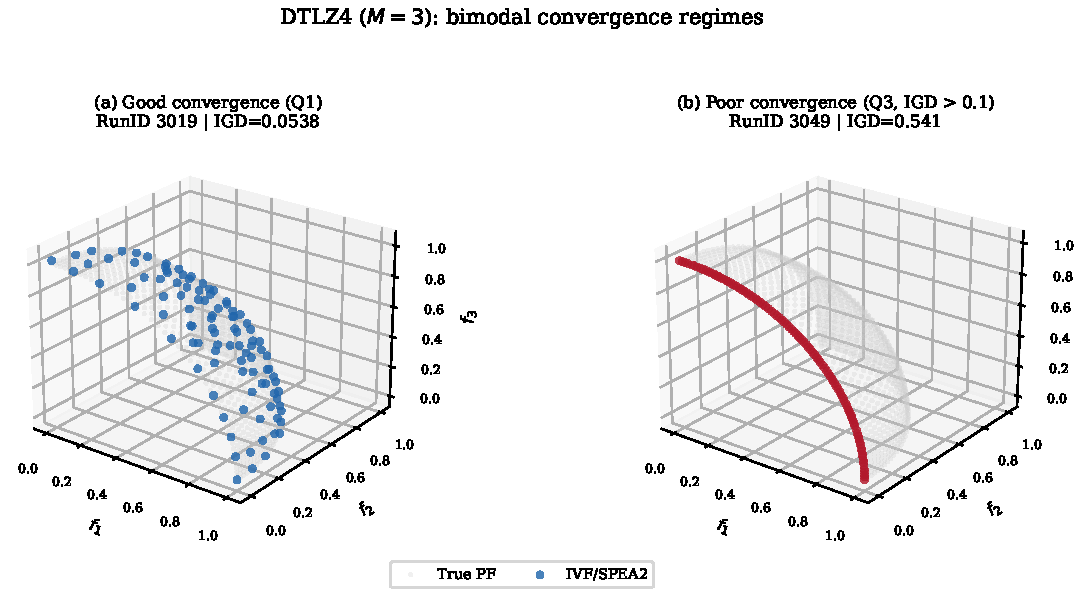
\includegraphics[width=0.86\textwidth]{../figures/dtlz4_bimodal_good_bad.pdf}
	\caption{DTLZ4 ($M=3$) bimodal convergence regimes under IVF/SPEA2. Representative runs were selected by a pre-defined criterion: good run with $\text{IGD} \leq Q_1$ and bad run with $\text{IGD} \geq Q_3$ and $\text{IGD} > 0.1$. For the 60-run cohort, $Q_1=5.39\times10^{-2}$ and $Q_3=5.41\times10^{-1}$, yielding the representative good and bad runs shown.}
	\label{fig:dtlz4-bimodal}
\end{figure*}

Representative success and failure fronts are shown in Fig.~\ref{fig:pareto-fronts} under the same median-IGD run criterion used across panels and algorithms. On DTLZ2, all methods track the reference front closely (success regime), whereas on WFG2 the IVF/SPEA2 cloud shows larger gaps and off-front dispersion than the comparators (failure regime).

\begin{figure*}[!htb]
	\centering
	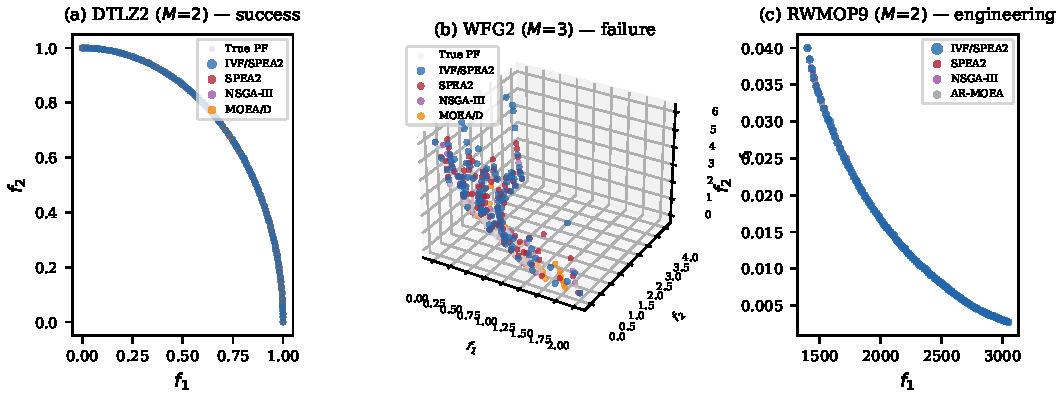
\includegraphics[width=0.92\textwidth]{../figures/pareto_fronts.pdf}
	\caption{Representative objective-space fronts from median-IGD runs. (a) DTLZ2 ($M=2$): IVF/SPEA2, SPEA2, NSGA-III, and MOEA/D all track the regular reference front (success regime). (b) WFG2 ($M=3$): IVF/SPEA2 shows visible gaps and off-front dispersion relative to SPEA2, NSGA-III, MOEA/D, and the disconnected reference structure (failure regime). (c) RWMOP9 ($M=2$): engineering comparison among IVF/SPEA2, SPEA2, NSGA-III, and AR-MOEA, illustrating the spread-quality trade-off discussed in Section~\ref{subsec:engineering}.}
	\label{fig:pareto-fronts}
\end{figure*}

The preceding figures show population-level outcomes; the next two zoom into individual IVF cycles. Fig.~\ref{fig:ivf-trace-panels} makes the operator-level mechanism directly observable on two pre-specified bi-objective trace cases: WFG7 ($M=2$), an out-of-sample Holm-supported gain, and WFG2 ($M=2$), a Holm-supported loss. For each case, 30 trace runs were generated; the displayed panel is cycle~1 from the run within one IGD interquartile range of the case median that has the most favorable or unfavorable median $\Delta d_{PF}$. On WFG7 (panel~a), the continuous front allows dissimilar-father selection to spread parents along different regions of the same front; in the selected cycle, 9 of 12 children (75\%) are closer to the reference front than their best parent. On WFG2 (panel~b), the inter-segment failure mode identified above is directly visible: all 12 children (100\%) are farther from the reference front than their best parent.

\begin{figure*}[!htb]
	\centering
	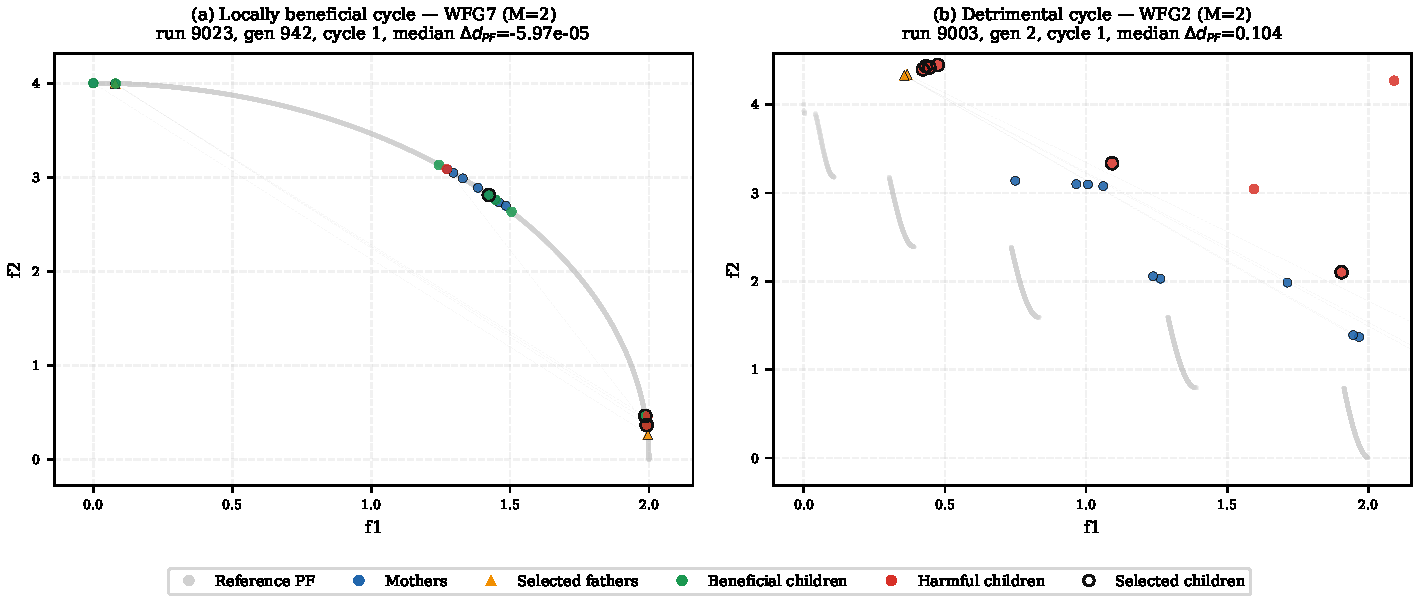
\includegraphics[width=0.92\textwidth]{../figures/ivf_trace_mechanistic_panels.pdf}
	\caption{Operator-level trace of cycle-1 episodes on bi-objective instances (panel selection protocol described in text). (a)~WFG7: mothers (blue) and dissimilar fathers (orange) span a continuous front; 75\% of children (green) improve over the best parent. (b)~WFG2: the same pairing rule crosses disconnected front segments; 100\% of children (red) degrade. Grey dots: reference front; black rings: children selected into the archive.}\label{fig:ivf-trace-panels}
\end{figure*}

A single cycle illustrates the mechanism but not its cumulative effect. Fig.~\ref{fig:ivf-trace-distance} therefore aggregates $\Delta d_{PF}$ over all IVF cycles across the same 30 traced runs per case as a function of dissimilar-father distance. On WFG7, the binned median stays near break-even regardless of parental distance, indicating that large H1 distances are not inherently harmful on a continuous front. On WFG2, the median is positive throughout and grows with distance, consistent with higher probability of crossing segment boundaries at larger separations. On DTLZ4 ($M=3$), the bimodal structure discussed above re-emerges: the cohort mixes convergent and non-convergent trajectories, yielding a positive median even at moderate distances.

\begin{figure*}[!htb]
	\centering
	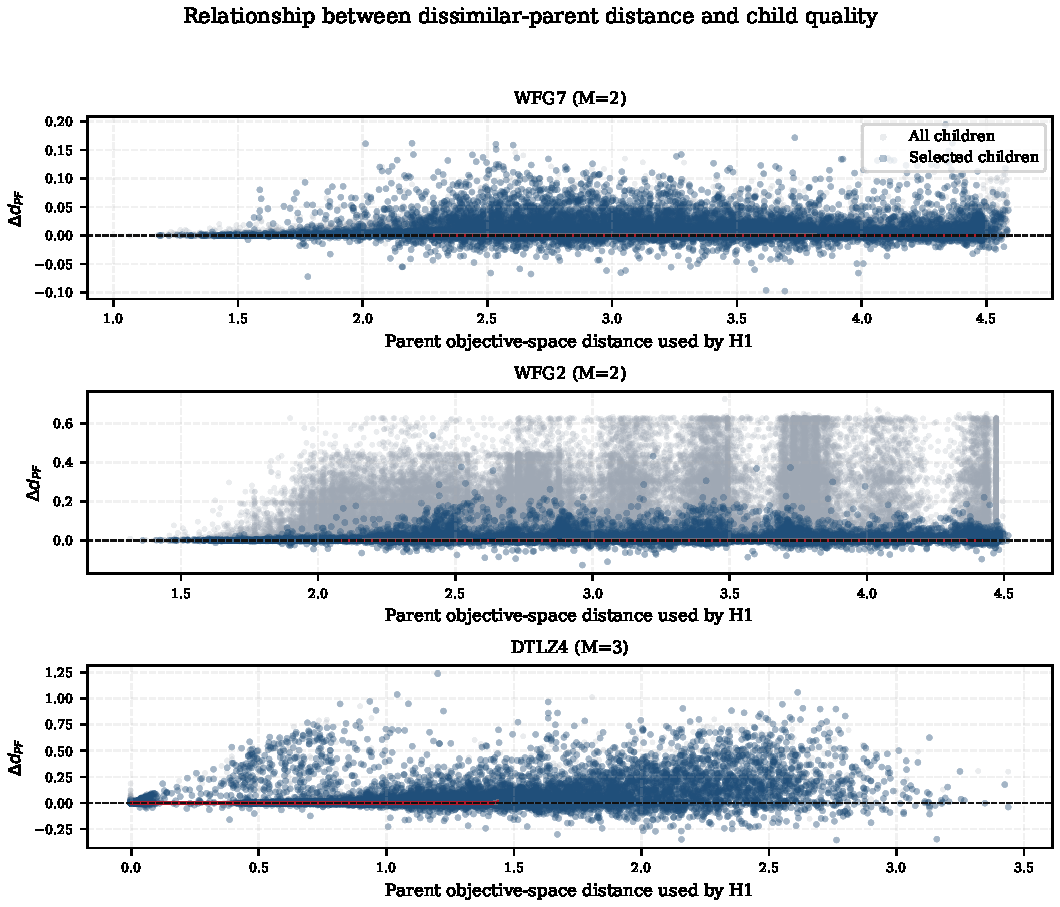
\includegraphics[width=0.92\textwidth]{../figures/ivf_trace_distance_vs_delta.pdf}
	\caption{Dissimilar-father distance versus offspring quality ($\Delta d_{PF}$) for the three trace cases (WFG7, WFG2, DTLZ4), aggregated over all IVF cycles across 30 runs per case. Grey dots: individual children; red curve: binned median; shaded band: interquartile range. Positive $\Delta d_{PF}$: child farther from the reference front than the best parent (harmful); dashed line: break-even.}\label{fig:ivf-trace-distance}
\end{figure*}

\subsection{Sensitivity and Tuning Implications}\label{subsec:discussion-sensitivity}
The tuning pipeline described in Section~\ref{subsec:sensitivity} yields two implications for practitioners. First, the absence of corrected IGD differences between C26 and A43 suggests that the EAR-PA mutation contribution and the execution/collection refinement affect partially separable aspects of the search process. After Holm--Bonferroni correction, the comparison is 0/12/0. This is weaker than a formal orthogonality claim, but it still indicates that useful performance can be obtained from more than one nearby operating point rather than from a single brittle configuration.

Second, the promoted C26 configuration functions as a robust operating point across the 12-problem tuning subset and generalizes to 39 out-of-sample instances, as reported in Section~\ref{subsec:results-spea2}, but it is not necessarily optimal for any single instance. The tuning landscape shown in Fig.~\ref{fig:sensitivity} corroborates this: the best-ranked cells in both Phase~A and Phase~C are surrounded by neighbours of comparable quality, and the Phase~B bar chart shows a clear separation between the winning operator profile and the stronger mutation variants, indicating that moderate deviations from the promoted default are unlikely to cause substantial degradation. In applications where maximizing absolute performance on a specific problem is required, instance-level retuning of $r$ and $c$ may yield further gains, particularly on landscapes where the default IVF intensity is either insufficient or excessive for the given front geometry.


\section{Conclusion}\label{sec:conclusion}

This work presents IVF/SPEA2 as a memetic hybrid whose effectiveness is governed by the interaction between IVF-generated offspring density and SPEA2's truncation mechanism. The main empirical pattern is geometric: IVF intensification is most beneficial on problems with regular Pareto-front structure, where SBX-generated offspring survive density-based archiving, and becomes less reliable on disconnected or irregular fronts, where those offspring are more likely to be removed by truncation.

The strongest generalization evidence comes from the 39 synthetic instances not used during tuning. On this out-of-sample subset, IVF/SPEA2 records IGD win/loss/tie counts of 20/2/2 for $M{=}2$ and 13/0/2 for $M{=}3$ under unadjusted Wilcoxon tests; after Holm--Bonferroni correction across all instances within each objective-count group, the counts remain 19/2/3 and 12/0/3. Over the full 51-instance synthetic suite, the corresponding corrected counts are 22/3/3 for $M{=}2$ and 15/1/7 for $M{=}3$. Hypervolume provides secondary support with the same qualitative scope limits. Taken together, these results indicate a bounded improvement over canonical SPEA2 at moderate objective counts rather than universal dominance.

The engineering study reinforces the same scope boundary. IVF/SPEA2 wins all IGD pairwise tests on RWMOP9, is balanced on RWMOP21, and is unfavorable on RWMOP8, which shows that transferability depends on constraint structure and objective-space geometry. Likewise, the DTLZ4 bimodal regime shows that non-significant rank tests can coexist with practically important dispersion, which is why the manuscript reports medians, IQR, and effect sizes rather than significance alone. From a practical standpoint, IVF/SPEA2 is most defensible when solution quality per fixed evaluation budget is the primary concern, since the budget-controlled protocol (Section~\ref{subsec:coupling}) adds only moderate algorithmic overhead.

The tuning arc closes without major contradictions. On the 12-problem tuning subset, the three-phase pipeline promotes configuration C26 with 4 corrected wins, 8 ties, and 0 losses against the original defaults. Under the production protocol, the same configuration retains strong out-of-sample performance, which supports its use as a stable default rather than as an instance-specific optimum.

Three follow-up directions emerge from the failure modes identified in Section~\ref{subsec:discussion-mechanism}. First, the WFG2/WFG9 losses suggest that \emph{topology-aware mating restriction} could reduce offspring placement in dominated inter-segment gaps. Specifically, the current front could be clustered in objective space and IVF crossover restricted to parents within the same segment; a lightweight online connectivity detector would make this adaptive without prior knowledge of front geometry. Second, the observation that IVF offspring on disconnected fronts are often rejected by density-based truncation motivates an \emph{adaptive IVF intensity} mechanism: monitoring offspring survival rates across generations and reducing the collection rate~$c$ or cycle count when survival drops below a threshold could preserve gains on regular fronts while limiting degradation on irregular ones. Third, because the primary failure mode appears to be the interaction between IVF-generated density and SPEA2's $k$-NN truncation rather than the IVF operator alone, \emph{host-transfer variants} should be evaluated on broader real-world and higher-dimensional benchmarks with $M>3$ objectives. These variants would couple IVF with alternative archiving strategies, such as $\varepsilon$-dominance archiving or reference-point-based selection. Overall, the present evidence supports IVF/SPEA2 as a conditional, host-specific improvement over SPEA2, with the clearest value on regular-front moderate-objective problems and weaker justification when front geometry is irregular.

\section*{Supplementary Information}

Supplementary Information~1 (PDF) contains the following material: the exploratory Friedman average-rank figure across all nine algorithms, representative engineering Pareto-front plots for RWMOP9, RWMOP21, and RWMOP8, and the supportive ablation tables and figure for the dissimilar-father and collective-cycle-continuation design refinements. Per-instance IGD and HV tables are provided in Appendix~\ref{app:tables}. All supplementary items use the same cohort filtering, testing rules, and sign conventions described in Section~\ref{subsec:stats}.

\backmatter

\bmhead{Acknowledgments}

Not applicable.

\section*{Statements and Declarations}

\begin{description}
	\item[Funding:] Not applicable.
	\item[Competing interests:] The authors declare no competing interests.
	\item[Ethics approval and consent to participate:] Not applicable.
	\item[Consent for publication:] Not applicable.
	\item[Data availability:] The processed benchmark results, manuscript tables, and reproducibility artifacts supporting this study are publicly available in the tagged IVF-SPEA2 release snapshot \citep{zambrano2026ivfspea2repo}. Additional raw experiment outputs are available from the corresponding author upon reasonable request.
	\item[Materials availability:] Not applicable.
	\item[Code availability:] The tagged IVF-SPEA2 release snapshot \citep{zambrano2026ivfspea2repo} contains the \texttt{IVFSPEA2V2} implementation, the frozen PlatEMO code used for the experiments, PlatEMO experiment runners, and the Python analysis scripts used to generate the reported tables and figures.
	\item[Author contributions:] Pedro Sanches Zambrano: conceptualization, methodology, software, investigation, formal analysis, data curation, writing (original draft). Eduardo Faria de Souza and Altino Dantas: co-supervision, validation, writing (review and editing). S\'avio Menezes Sampaio: conceptualization, data curation, co-supervision, validation, writing (review and editing). Celso G. Camilo-Junior: supervision, project administration, methodology guidance, writing (review and editing).
\end{description}


\bibliography{../bib/sn-bibliography}% common bib file
%%\input sn-article.bbl

\appendix

\section{Per-Instance IGD and HV Tables}\label{app:tables}

Tables~\ref{tab:igd_per_instance_m2}--\ref{tab:hv_per_instance_m3} report the median and interquartile range of IGD and HV for all synthetic instances. Significance symbols follow the same conventions as the main text (Wilcoxon rank-sum, $\alpha=0.05$, from IVF/SPEA2's perspective). Several algorithm--instance combinations exhibit IQR values that are orders of magnitude larger than the corresponding median (e.g., MOEA/D on DTLZ7/MaF7, AR-MOEA on DTLZ4 at $M{=}2$, and multiple algorithms on MaF5). These extreme IQR values reflect bimodal or multi-modal convergence behavior in which a substantial fraction of the 60 runs fails to reach the Pareto front, producing a mixture of low- and high-IGD outcomes. The IVF/SPEA2 case on DTLZ4 ($M{=}3$) is discussed in Section~\ref{subsec:discussion-mechanism}; the remaining cases are not specific to IVF and are consistent with known difficulty profiles of the respective benchmark--algorithm pairings.

\begin{landscape}
	{\tiny
		\setlength{\tabcolsep}{2pt}%
		\renewcommand{\arraystretch}{0.95}%
		\begin{longtable}{llrrrrrrrrr}
			\caption{Median IGD (IQR) across all $M=2$ instances over 60 independent runs. Symbols indicate Wilcoxon rank-sum test ($\alpha=0.05$) of IVF/SPEA2 vs.\ each baseline: $+$ (IVF/SPEA2 significantly better, i.e.\ lower IGD), $-$ (significantly worse), $\approx$ (no significant difference). Best median per instance in \textbf{bold}.}
			\label{tab:igd_per_instance_m2}                                                                                                                                                                                                                                                                                         \\
			\toprule
			Problem                           & $D$ & IVF/SPEA2              & SPEA2                              & MFO-SPEA2                    & SPEA2+SDE                 & NSGA-II                   & NSGA-III                     & MOEA/D                       & AGE-II                       & AR-MOEA                     \\
			\midrule
			\endfirsthead
			\multicolumn{11}{c}{{\textit{Continued from previous page}}}                                                                                                                                                                                                                                                            \\
			\toprule
			Problem                           & $D$ & IVF/SPEA2              & SPEA2                              & MFO-SPEA2                    & SPEA2+SDE                 & NSGA-II                   & NSGA-III                     & MOEA/D                       & AGE-II                       & AR-MOEA                     \\
			\midrule
			\endhead
			\midrule
			\multicolumn{11}{r}{{\textit{Continued on next page}}}                                                                                                                                                                                                                                                                  \\
			\endfoot
			\botrule
			\endlastfoot
			ZDT1                              & 30  & \textbf{3.88(0.09)e-3} & 3.97(0.11)e-3$^{+}$                & 3.93(0.08)e-3$^{+}$          & 4.24(0.20)e-3$^{+}$       & 4.81(0.27)e-3$^{+}$       & 3.89(0.00)e-3$^{\approx}$    & 3.99(0.05)e-3$^{+}$          & 4.62(0.13)e-3$^{+}$          & 3.89(0.00)e-3$^{\approx}$   \\
			ZDT2                              & 30  & 3.89(0.06)e-3          & 3.91(0.06)e-3$^{+}$                & 3.93(0.06)e-3$^{+}$          & 6.02(0.86)e-3$^{+}$       & 4.88(0.31)e-3$^{+}$       & \textbf{3.81(0.00)e-3}$^{-}$ & 4.00(0.10)e-3$^{+}$          & 4.69(0.19)e-3$^{+}$          & 3.81(0.00)e-3$^{-}$         \\
			ZDT3                              & 30  & \textbf{4.84(0.11)e-3} & 4.92(0.18)e-3$^{+}$                & 4.89(0.13)e-3$^{+}$          & 5.30(0.28)e-3$^{+}$       & 5.43(0.27)e-3$^{+}$       & 6.13(0.21)e-3$^{+}$          & 1.21(0.06)e-2$^{+}$          & 5.77(0.08)e-3$^{+}$          & 6.44(0.01)e-3$^{+}$         \\
			ZDT4                              & 10  & \textbf{3.81(0.04)e-3} & 3.86(0.05)e-3$^{+}$                & 3.83(0.04)e-3$^{+}$          & 4.25(0.15)e-3$^{+}$       & 4.54(0.23)e-3$^{+}$       & 3.89(0.02)e-3$^{+}$          & 4.84(0.72)e-3$^{+}$          & 4.56(0.16)e-3$^{+}$          & 3.90(0.02)e-3$^{+}$         \\
			ZDT6                              & 10  & 3.06(0.03)e-3          & 3.10(0.03)e-3$^{+}$                & 3.08(0.03)e-3$^{+}$          & 3.43(0.08)e-3$^{+}$       & 3.67(0.18)e-3$^{+}$       & \textbf{3.00(0.00)e-3}$^{-}$ & 3.54(0.25)e-3$^{+}$          & 3.62(0.10)e-3$^{+}$          & 3.00(0.00)e-3$^{-}$         \\
			\midrule
			DTLZ1                             & 6   & 1.83(0.01)e-3          & 1.83(0.01)e-3$^{+}$                & 1.84(0.02)e-3$^{+}$          & 2.00(0.07)e-3$^{+}$       & 2.21(0.08)e-3$^{+}$       & \textbf{1.79(0.00)e-3}$^{-}$ & 1.79(0.00)e-3$^{-}$          & 2.03(0.09)e-3$^{+}$          & 1.79(0.00)e-3$^{-}$         \\
			DTLZ2                             & 11  & 4.12(0.06)e-3          & 4.18(0.06)e-3$^{+}$                & 4.17(0.07)e-3$^{+}$          & 9.67(0.92)e-3$^{+}$       & 5.12(0.22)e-3$^{+}$       & 3.97(0.00)e-3$^{-}$          & \textbf{3.97(0.00)e-3}$^{-}$ & 4.50(0.07)e-3$^{+}$          & 3.97(0.00)e-3$^{-}$         \\
			DTLZ3                             & 11  & \textbf{4.05(0.05)e-3} & 4.29(0.38)e-3$^{+}$                & 4.28(0.29)e-3$^{+}$          & 1.01(0.14)e-2$^{+}$       & 5.31(0.51)e-3$^{+}$       & 4.22(0.53)e-3$^{+}$          & 4.40(0.69)e-3$^{+}$          & 4.54(0.14)e-3$^{+}$          & 4.22(0.34)e-3$^{+}$         \\
			DTLZ4                             & 11  & 4.11(0.08)e-3          & 4.16(0.08)e-3$^{+}$                & 4.17(0.09)e-3$^{+}$          & 9.83(2.28)e-3$^{+}$       & 5.20(0.46)e-3$^{+}$       & 3.97(0.00)e-3$^{-}$          & \textbf{3.97(0.00)e-3}$^{-}$ & 4.53(0.21)e-3$^{+}$          & 3.99(738.12)e-3$^{\approx}$ \\
			DTLZ5                             & 11  & 4.12(0.05)e-3          & 4.17(0.06)e-3$^{+}$                & 4.17(0.06)e-3$^{+}$          & 1.00(0.18)e-2$^{+}$       & 5.03(0.25)e-3$^{+}$       & 3.97(0.00)e-3$^{-}$          & \textbf{3.97(0.00)e-3}$^{-}$ & 4.48(0.05)e-3$^{+}$          & 3.97(0.00)e-3$^{-}$         \\
			DTLZ6                             & 11  & 4.06(0.05)e-3          & 4.09(0.04)e-3$^{+}$                & 4.09(0.05)e-3$^{+}$          & 9.51(1.24)e-3$^{+}$       & 5.65(0.40)e-3$^{+}$       & 3.97(0.00)e-3$^{-}$          & \textbf{3.97(0.00)e-3}$^{-}$ & 4.46(0.05)e-3$^{+}$          & 3.97(0.00)e-3$^{-}$         \\
			DTLZ7                             & 21  & \textbf{4.73(0.12)e-3} & 4.77(0.13)e-3$^{+}$                & 4.73(0.13)e-3$^{\approx}$    & 5.25(0.24)e-3$^{+}$       & 5.38(0.30)e-3$^{+}$       & 5.12(0.11)e-3$^{+}$          & 7.40(437.83)e-3$^{+}$        & 5.24(0.20)e-3$^{+}$          & 5.05(0.01)e-3$^{+}$         \\
			\midrule
			WFG1                              & 11  & 2.22(1.52)e-2          & 2.93(2.40)e-2$^{+}$                & 1.09(0.06)e-1$^{+}$          & 4.08(3.66)e-2$^{+}$       & 2.15(0.19)e-2$^{\approx}$ & 9.69(2.12)e-2$^{+}$          & 3.29(1.34)e-2$^{+}$          & \textbf{1.99(0.16)e-2}$^{-}$ & 1.04(0.23)e-1$^{+}$         \\
			WFG2                              & 11  & 1.14(0.06)e-2          & 1.11(0.02)e-2$^{-}$                & \textbf{1.10(0.02)e-2}$^{-}$ & 1.36(0.09)e-2$^{+}$       & 1.29(0.05)e-2$^{+}$       & 1.38(0.08)e-2$^{+}$          & 4.31(0.18)e-2$^{+}$          & 1.44(0.08)e-2$^{+}$          & 1.32(0.01)e-2$^{+}$         \\
			WFG3                              & 11  & 1.23(0.06)e-2          & 1.20(0.03)e-2$^{-}$                & 1.20(0.03)e-2$^{-}$          & 1.31(0.04)e-2$^{+}$       & 1.45(0.06)e-2$^{+}$       & \textbf{1.13(0.01)e-2}$^{-}$ & 1.38(0.03)e-2$^{+}$          & 1.32(0.04)e-2$^{+}$          & 1.14(0.01)e-2$^{-}$         \\
			WFG4                              & 11  & 1.26(0.02)e-2          & 1.29(0.03)e-2$^{+}$                & 1.29(0.02)e-2$^{+}$          & 3.23(0.77)e-2$^{+}$       & 1.53(0.06)e-2$^{+}$       & \textbf{1.22(0.00)e-2}$^{-}$ & 1.59(0.19)e-2$^{+}$          & 1.38(0.03)e-2$^{+}$          & 1.22(0.00)e-2$^{-}$         \\
			WFG5                              & 11  & 6.35(0.01)e-2          & 6.37(0.01)e-2$^{+}$                & 6.37(0.02)e-2$^{+}$          & 7.57(0.56)e-2$^{+}$       & 6.53(0.05)e-2$^{+}$       & \textbf{6.34(0.00)e-2}$^{-}$ & 6.98(0.03)e-2$^{+}$          & 6.40(0.01)e-2$^{+}$          & 6.34(0.01)e-2$^{\approx}$   \\
			WFG6                              & 11  & 8.31(3.63)e-2          & \textbf{7.64(2.94)e-2}$^{\approx}$ & 8.59(2.78)e-2$^{\approx}$    & 9.04(3.39)e-2$^{\approx}$ & 8.19(2.61)e-2$^{\approx}$ & 8.30(2.86)e-2$^{\approx}$    & 8.18(3.16)e-2$^{\approx}$    & 7.77(3.30)e-2$^{\approx}$    & 7.69(2.98)e-2$^{\approx}$   \\
			WFG7                              & 11  & 1.32(0.03)e-2          & 1.37(0.05)e-2$^{+}$                & 1.37(0.04)e-2$^{+}$          & 3.20(0.54)e-2$^{+}$       & 1.70(0.09)e-2$^{+}$       & \textbf{1.22(0.00)e-2}$^{-}$ & 1.54(0.13)e-2$^{+}$          & 1.39(0.03)e-2$^{+}$          & 1.22(0.00)e-2$^{-}$         \\
			WFG8                              & 11  & 1.07(0.02)e-1          & 1.07(0.02)e-1$^{\approx}$          & 1.07(0.02)e-1$^{\approx}$    & 1.13(0.04)e-1$^{+}$       & 1.09(0.02)e-1$^{+}$       & \textbf{1.05(0.02)e-1}$^{-}$ & 1.09(0.04)e-1$^{+}$          & 1.06(0.03)e-1$^{-}$          & 1.06(0.02)e-1$^{-}$         \\
			WFG9                              & 11  & 1.69(0.36)e-2          & 1.59(0.14)e-2$^{-}$                & 1.55(0.16)e-2$^{-}$          & 3.24(0.67)e-2$^{+}$       & 1.85(0.17)e-2$^{+}$       & \textbf{1.45(0.19)e-2}$^{-}$ & 3.10(0.42)e-2$^{+}$          & 1.60(0.15)e-2$^{-}$          & 1.55(0.16)e-2$^{-}$         \\
			\midrule
			MaF1                              & 11  & 3.74(0.05)e-3          & 3.80(0.06)e-3$^{+}$                & 3.80(0.07)e-3$^{+}$          & 3.98(0.09)e-3$^{+}$       & 4.63(0.17)e-3$^{+}$       & 3.57(0.00)e-3$^{-}$          & \textbf{3.57(0.00)e-3}$^{-}$ & 4.06(0.11)e-3$^{+}$          & 3.57(0.00)e-3$^{-}$         \\
			MaF2                              & 11  & 2.11(0.03)e-3          & 2.19(0.04)e-3$^{+}$                & 2.18(0.04)e-3$^{+}$          & 2.38(0.11)e-3$^{+}$       & 2.76(0.19)e-3$^{+}$       & \textbf{2.01(0.00)e-3}$^{-}$ & 2.01(0.01)e-3$^{-}$          & 2.54(0.03)e-3$^{+}$          & 2.01(0.00)e-3$^{-}$         \\
			MaF3                              & 11  & \textbf{3.77(0.07)e-3} & 4.20(0.64)e-3$^{+}$                & 4.39(0.84)e-3$^{+}$          & 7.76(1.98)e-3$^{+}$       & 4.91(0.45)e-3$^{+}$       & 6.43(0.54)e-3$^{+}$          & 1.12(0.26)e-2$^{+}$          & 4.75(0.36)e-3$^{+}$          & 6.48(0.69)e-3$^{+}$         \\
			MaF4                              & 11  & \textbf{1.25(0.01)e-2} & 1.27(0.02)e-2$^{+}$                & 1.26(0.03)e-2$^{+}$          & 4.09(1.43)e-2$^{+}$       & 1.55(0.09)e-2$^{+}$       & 3.51(0.03)e-2$^{+}$          & 1.87(0.02)e-1$^{+}$          & 1.48(0.05)e-2$^{+}$          & 3.51(0.03)e-2$^{+}$         \\
			MaF5                              & 11  & 1.27(0.03)e-2          & 1.29(0.04)e-2$^{+}$                & 1.29(0.03)e-2$^{+}$          & 3.28(0.81)e-2$^{+}$       & 1.60(199.31)e-2$^{+}$     & \textbf{1.22(0.00)e-2}$^{-}$ & 1.31(0.00)e-2$^{+}$          & 1.40(0.06)e-2$^{+}$          & 1.22(199.61)e-2$^{-}$       \\
			MaF6                              & 11  & 4.05(0.03)e-3          & 4.09(0.05)e-3$^{+}$                & 4.08(0.04)e-3$^{+}$          & 1.00(0.15)e-2$^{+}$       & 4.96(0.19)e-3$^{+}$       & 3.97(0.00)e-3$^{-}$          & \textbf{3.97(0.00)e-3}$^{-}$ & 4.49(0.09)e-3$^{+}$          & 3.97(0.00)e-3$^{-}$         \\
			MaF7                              & 21  & \textbf{4.72(0.12)e-3} & 4.78(0.16)e-3$^{+}$                & 4.76(0.13)e-3$^{\approx}$    & 5.18(0.28)e-3$^{+}$       & 5.43(0.30)e-3$^{+}$       & 5.12(0.10)e-3$^{+}$          & 7.38(437.90)e-3$^{+}$        & 5.23(0.16)e-3$^{+}$          & 5.05(0.01)e-3$^{+}$         \\
			\midrule
			\multicolumn{2}{l}{$+/\approx/-$} & --- & 23/2/3                 & 21/4/3                             & 27/1/0                       & 26/2/0                    & 9/2/17                    & 19/1/8                       & 24/1/3                       & 9/4/15                                                     \\
		\end{longtable}
	}
\end{landscape}

\clearpage
\begin{landscape}
	{\tiny
		\setlength{\tabcolsep}{2pt}%
		\renewcommand{\arraystretch}{0.95}%
		\begin{longtable}{llrrrrrrrrr}
			\caption{Median IGD (IQR) across all $M=3$ instances over 60 independent runs. Symbols as in Table~\ref{tab:igd_per_instance_m2}.}
			\label{tab:igd_per_instance_m3}                                                                                                                                                                                                                                                                                                        \\
			\toprule
			Problem                           & $D$ & IVF/SPEA2              & SPEA2                      & MFO-SPEA2                          & SPEA2+SDE                          & NSGA-II                   & NSGA-III                     & MOEA/D                        & AGE-II                             & AR-MOEA                      \\
			\midrule
			\endfirsthead
			\multicolumn{11}{c}{{\textit{Continued from previous page}}}                                                                                                                                                                                                                                                                           \\
			\toprule
			Problem                           & $D$ & IVF/SPEA2              & SPEA2                      & MFO-SPEA2                          & SPEA2+SDE                          & NSGA-II                   & NSGA-III                     & MOEA/D                        & AGE-II                             & AR-MOEA                      \\
			\midrule
			\endhead
			\midrule
			\multicolumn{11}{r}{{\textit{Continued on next page}}}                                                                                                                                                                                                                                                                                 \\
			\endfoot
			\botrule
			\endlastfoot
			DTLZ1                             & 7   & 2.01(0.02)e-2          & 2.01(0.02)e-2$^{\approx}$  & 2.02(0.02)e-2$^{+}$                & 2.06(0.03)e-2$^{+}$                & 2.68(0.15)e-2$^{+}$       & 2.06(0.00)e-2$^{+}$          & 2.06(0.00)e-2$^{+}$           & \textbf{2.00(0.01)e-2}$^{\approx}$ & 2.06(0.00)e-2$^{+}$          \\
			DTLZ2                             & 12  & 5.37(0.07)e-2          & 5.42(0.07)e-2$^{+}$        & 5.42(0.08)e-2$^{+}$                & 7.68(0.30)e-2$^{+}$                & 6.87(0.32)e-2$^{+}$       & 5.45(0.00)e-2$^{+}$          & 5.45(0.00)e-2$^{+}$           & \textbf{5.26(0.10)e-2}$^{-}$       & 5.45(0.00)e-2$^{+}$          \\
			DTLZ3                             & 12  & 5.30(0.08)e-2          & 5.33(0.06)e-2$^{+}$        & 5.35(0.08)e-2$^{+}$                & 7.55(0.34)e-2$^{+}$                & 6.91(0.45)e-2$^{+}$       & 5.46(0.03)e-2$^{+}$          & 5.46(0.02)e-2$^{+}$           & \textbf{5.28(0.05)e-2}$^{-}$       & 5.46(0.03)e-2$^{+}$          \\
			DTLZ4                             & 12  & 5.45(48.70)e-2         & 5.50(48.63)e-2$^{+}$       & 5.49(0.10)e-2$^{\approx}$          & 7.90(0.66)e-2$^{+}$                & 6.77(0.23)e-2$^{\approx}$ & 5.45(0.00)e-2$^{\approx}$    & \textbf{5.45(48.71)e-2}$^{-}$ & 5.57(0.39)e-2$^{\approx}$          & 5.45(48.64)e-2$^{+}$         \\
			DTLZ5                             & 12  & \textbf{4.28(0.13)e-3} & 4.41(0.14)e-3$^{+}$        & 4.40(0.13)e-3$^{+}$                & 9.84(1.57)e-3$^{+}$                & 5.80(0.36)e-3$^{+}$       & 1.29(0.21)e-2$^{+}$          & 3.39(0.00)e-2$^{+}$           & 1.12(0.59)e-2$^{+}$                & 5.37(0.15)e-3$^{+}$          \\
			DTLZ6                             & 12  & \textbf{4.05(0.05)e-3} & 4.08(0.03)e-3$^{+}$        & 4.08(0.04)e-3$^{+}$                & 9.67(1.63)e-3$^{+}$                & 5.83(0.39)e-3$^{+}$       & 1.82(0.25)e-2$^{+}$          & 3.39(0.00)e-2$^{+}$           & 7.39(0.03)e-3$^{+}$                & 5.00(0.09)e-3$^{+}$          \\
			DTLZ7                             & 22  & 6.00(0.14)e-2          & 6.06(0.18)e-2$^{+}$        & 6.04(0.17)e-2$^{\approx}$          & \textbf{5.99(0.60)e-2}$^{\approx}$ & 7.72(0.57)e-2$^{+}$       & 7.59(0.50)e-2$^{+}$          & 1.54(0.02)e-1$^{+}$           & 6.06(0.21)e-2$^{+}$                & 6.82(7.31)e-2$^{+}$          \\
			\midrule
			WFG1                              & 12  & 1.52(0.05)e-1          & 1.53(0.06)e-1$^{\approx}$  & 1.52(0.05)e-1$^{\approx}$          & 1.75(0.17)e-1$^{+}$                & 2.23(0.13)e-1$^{+}$       & \textbf{1.48(0.02)e-1}$^{-}$ & 2.28(0.08)e-1$^{+}$           & 1.49(0.03)e-1$^{-}$                & 1.49(0.04)e-1$^{-}$          \\
			WFG2                              & 12  & 1.82(0.08)e-1          & 1.73(0.06)e-1$^{-}$        & 1.67(0.06)e-1$^{-}$                & 2.06(0.14)e-1$^{+}$                & 2.20(0.19)e-1$^{+}$       & 1.65(0.01)e-1$^{-}$          & 2.40(0.06)e-1$^{+}$           & 1.73(0.05)e-1$^{-}$                & \textbf{1.64(0.02)e-1}$^{-}$ \\
			WFG3                              & 12  & 8.75(1.04)e-2          & 9.62(0.99)e-2$^{+}$        & 1.05(0.11)e-1$^{+}$                & \textbf{6.44(0.87)e-2}$^{-}$       & 8.93(1.57)e-2$^{\approx}$ & 1.05(0.16)e-1$^{+}$          & 1.57(0.01)e-1$^{+}$           & 6.54(0.48)e-2$^{-}$                & 1.17(0.11)e-1$^{+}$          \\
			WFG4                              & 12  & \textbf{2.12(0.03)e-1} & 2.15(0.03)e-1$^{+}$        & 2.15(0.04)e-1$^{+}$                & 3.22(0.18)e-1$^{+}$                & 2.70(0.12)e-1$^{+}$       & 2.21(0.00)e-1$^{+}$          & 2.53(0.04)e-1$^{+}$           & 2.13(0.07)e-1$^{\approx}$          & 2.21(0.00)e-1$^{+}$          \\
			WFG5                              & 12  & \textbf{2.21(0.02)e-1} & 2.23(0.02)e-1$^{+}$        & 2.23(0.03)e-1$^{+}$                & 3.34(0.19)e-1$^{+}$                & 2.77(0.13)e-1$^{+}$       & 2.30(0.00)e-1$^{+}$          & 2.48(0.03)e-1$^{+}$           & 2.33(0.15)e-1$^{+}$                & 2.30(0.00)e-1$^{+}$          \\
			WFG6                              & 12  & 2.38(0.16)e-1          & 2.39(0.14)e-1$^{\approx}$  & 2.41(0.14)e-1$^{\approx}$          & 3.39(0.20)e-1$^{+}$                & 3.04(0.20)e-1$^{+}$       & 2.38(0.12)e-1$^{\approx}$    & 2.70(0.11)e-1$^{+}$           & \textbf{2.32(0.15)e-1}$^{-}$       & 2.39(0.10)e-1$^{\approx}$    \\
			WFG7                              & 12  & \textbf{2.14(0.04)e-1} & 2.17(0.04)e-1$^{+}$        & 2.18(0.04)e-1$^{+}$                & 3.28(0.20)e-1$^{+}$                & 2.78(0.12)e-1$^{+}$       & 2.21(0.00)e-1$^{+}$          & 2.91(0.24)e-1$^{+}$           & 2.14(0.08)e-1$^{\approx}$          & 2.21(0.00)e-1$^{+}$          \\
			WFG8                              & 12  & 2.93(0.06)e-1          & 2.95(0.07)e-1$^{+}$        & 2.98(0.06)e-1$^{+}$                & 3.57(0.17)e-1$^{+}$                & 3.73(0.17)e-1$^{+}$       & 2.79(0.04)e-1$^{-}$          & 3.03(0.07)e-1$^{+}$           & 2.88(0.07)e-1$^{-}$                & \textbf{2.71(0.02)e-1}$^{-}$ \\
			WFG9                              & 12  & \textbf{2.10(0.04)e-1} & 2.17(0.05)e-1$^{+}$        & 2.17(0.05)e-1$^{+}$                & 3.12(0.14)e-1$^{+}$                & 2.73(0.14)e-1$^{+}$       & 2.22(0.01)e-1$^{+}$          & 2.56(0.21)e-1$^{+}$           & 2.13(0.05)e-1$^{+}$                & 2.21(0.01)e-1$^{+}$          \\
			\midrule
			MaF1                              & 12  & 4.11(0.05)e-2          & 4.17(0.06)e-2$^{+}$        & 4.19(0.05)e-2$^{+}$                & 4.20(0.09)e-2$^{+}$                & 5.71(0.34)e-2$^{+}$       & 6.07(0.26)e-2$^{+}$          & 7.05(0.00)e-2$^{+}$           & \textbf{3.99(0.03)e-2}$^{-}$       & 4.36(0.05)e-2$^{+}$          \\
			MaF2                              & 12  & 3.11(0.15)e-2          & 3.23(0.14)e-2$^{+}$        & 3.09(0.14)e-2$^{\approx}$          & 3.12(0.08)e-2$^{\approx}$          & 4.56(0.47)e-2$^{+}$       & 3.60(0.06)e-2$^{+}$          & 3.89(0.08)e-2$^{+}$           & \textbf{2.96(0.05)e-2}$^{-}$       & 3.29(0.10)e-2$^{+}$          \\
			MaF3                              & 12  & \textbf{3.25(0.05)e-2} & 3.33(0.08)e-2$^{+}$        & 3.34(0.10)e-2$^{+}$                & 5.91(0.92)e-2$^{+}$                & 5.64(2.06)e-2$^{+}$       & 4.70(0.10)e-2$^{+}$          & 5.23(0.21)e-2$^{+}$           & 3.40(0.08)e-2$^{+}$                & 4.69(0.05)e-2$^{+}$          \\
			MaF4                              & 12  & \textbf{2.39(0.04)e-1} & 2.42(0.04)e-1$^{+}$        & 2.41(0.04)e-1$^{+}$                & 4.63(1.24)e-1$^{+}$                & 2.96(0.13)e-1$^{+}$       & 3.38(0.24)e-1$^{+}$          & 6.82(0.39)e-1$^{+}$           & 2.91(0.13)e-1$^{+}$                & 3.42(0.04)e-1$^{+}$          \\
			MaF5                              & 12  & 2.48(12.49)e-1         & 2.47(12.47)e-1$^{\approx}$ & \textbf{2.46(0.05)e-1}$^{\approx}$ & 3.73(3.10)e-1$^{+}$                & 3.01(0.17)e-1$^{\approx}$ & 2.60(12.40)e-1$^{+}$         & 2.97(0.00)e-1$^{\approx}$     & 2.59(0.23)e-1$^{\approx}$          & 2.60(13.65)e-1$^{+}$         \\
			MaF6                              & 12  & \textbf{4.05(0.04)e-3} & 4.09(0.04)e-3$^{+}$        & 4.08(0.05)e-3$^{+}$                & 9.57(1.27)e-3$^{+}$                & 5.24(0.35)e-3$^{+}$       & 1.52(0.26)e-2$^{+}$          & 3.39(0.00)e-2$^{+}$           & 5.31(0.46)e-3$^{+}$                & 5.05(0.13)e-3$^{+}$          \\
			MaF7                              & 22  & 5.94(0.15)e-2          & 6.01(0.17)e-2$^{+}$        & 6.04(0.23)e-2$^{+}$                & \textbf{5.92(0.39)e-2}$^{\approx}$ & 7.67(0.66)e-2$^{+}$       & 7.61(0.52)e-2$^{+}$          & 1.54(0.01)e-1$^{+}$           & 6.10(0.13)e-2$^{+}$                & 6.87(28.00)e-2$^{+}$         \\
			\midrule
			\multicolumn{2}{l}{$+/\approx/-$} & --- & 18/4/1                 & 16/6/1                     & 19/3/1                             & 20/3/0                             & 18/2/3                    & 21/1/1                       & 9/5/9                         & 19/1/3                                                            \\
		\end{longtable}
	}
\end{landscape}

\clearpage
\begin{landscape}
	{\tiny
		\setlength{\tabcolsep}{2pt}%
		\renewcommand{\arraystretch}{0.95}%
		\begin{longtable}{llrrrrrrrrr}
			\caption{Median HV (IQR) across all $M=2$ instances over 60 independent runs. Symbols indicate Wilcoxon rank-sum test ($\alpha=0.05$) of IVF/SPEA2 vs.\ each baseline: $+$ (IVF/SPEA2 significantly better, i.e.\ higher HV), $-$ (significantly worse), $\approx$ (no significant difference). Best median per instance in \textbf{bold}.}
			\label{tab:hv_per_instance_m2}                                                                                                                                                                                                                                                                                                 \\
			\toprule
			Problem                           & $D$ & IVF/SPEA2              & SPEA2                              & MFO-SPEA2                    & SPEA2+SDE                 & NSGA-II                      & NSGA-III                           & MOEA/D                       & AGE-II                       & AR-MOEA                   \\
			\midrule
			\endfirsthead
			\multicolumn{11}{c}{{\textit{Continued from previous page}}}                                                                                                                                                                                                                                                                   \\
			\toprule
			Problem                           & $D$ & IVF/SPEA2              & SPEA2                              & MFO-SPEA2                    & SPEA2+SDE                 & NSGA-II                      & NSGA-III                           & MOEA/D                       & AGE-II                       & AR-MOEA                   \\
			\midrule
			\endhead
			\midrule
			\multicolumn{11}{r}{{\textit{Continued on next page}}}                                                                                                                                                                                                                                                                         \\
			\endfoot
			\botrule
			\endlastfoot
			ZDT1                              & 30  & \textbf{7.20(0.00)e-1} & 7.20(0.00)e-1$^{+}$                & 7.20(0.00)e-1$^{+}$          & 7.20(0.00)e-1$^{+}$       & 7.19(0.00)e-1$^{+}$          & 7.20(0.00)e-1$^{+}$                & 7.19(0.00)e-1$^{+}$          & 7.20(0.00)e-1$^{+}$          & 7.20(0.00)e-1$^{+}$       \\
			ZDT2                              & 30  & 4.45(0.00)e-1          & 4.45(0.00)e-1$^{+}$                & 4.45(0.00)e-1$^{+}$          & 4.45(0.00)e-1$^{+}$       & 4.44(0.00)e-1$^{+}$          & \textbf{4.45(0.00)e-1}$^{\approx}$ & 4.44(0.00)e-1$^{+}$          & 4.44(0.00)e-1$^{+}$          & 4.45(0.00)e-1$^{\approx}$ \\
			ZDT3                              & 30  & \textbf{6.00(0.00)e-1} & 6.00(0.00)e-1$^{+}$                & 6.00(0.00)e-1$^{+}$          & 5.99(0.00)e-1$^{+}$       & 5.99(0.00)e-1$^{+}$          & 5.99(0.00)e-1$^{+}$                & 5.97(0.01)e-1$^{+}$          & 5.99(0.00)e-1$^{+}$          & 5.99(0.00)e-1$^{+}$       \\
			ZDT4                              & 10  & \textbf{7.21(0.00)e-1} & 7.20(0.00)e-1$^{+}$                & 7.20(0.00)e-1$^{+}$          & 7.19(0.00)e-1$^{+}$       & 7.20(0.00)e-1$^{+}$          & 7.20(0.00)e-1$^{+}$                & 7.17(0.02)e-1$^{+}$          & 7.20(0.00)e-1$^{+}$          & 7.20(0.00)e-1$^{+}$       \\
			ZDT6                              & 10  & 3.89(0.00)e-1          & 3.89(0.00)e-1$^{+}$                & 3.89(0.00)e-1$^{+}$          & 3.89(0.00)e-1$^{+}$       & 3.88(0.00)e-1$^{+}$          & \textbf{3.89(0.00)e-1}$^{-}$       & 3.88(0.01)e-1$^{+}$          & 3.88(0.00)e-1$^{+}$          & 3.89(0.00)e-1$^{-}$       \\
			\midrule
			DTLZ1                             & 6   & 5.83(0.00)e-1          & 5.82(0.00)e-1$^{+}$                & 5.82(0.00)e-1$^{+}$          & 5.82(0.00)e-1$^{+}$       & 5.81(0.00)e-1$^{+}$          & \textbf{5.83(0.00)e-1}$^{-}$       & 5.83(0.00)e-1$^{-}$          & 5.82(0.00)e-1$^{+}$          & 5.83(0.00)e-1$^{\approx}$ \\
			DTLZ2                             & 11  & \textbf{3.47(0.00)e-1} & 3.47(0.00)e-1$^{+}$                & 3.47(0.00)e-1$^{+}$          & 3.47(0.00)e-1$^{+}$       & 3.47(0.00)e-1$^{+}$          & 3.47(0.00)e-1$^{+}$                & 3.47(0.00)e-1$^{+}$          & 3.47(0.00)e-1$^{+}$          & 3.47(0.00)e-1$^{+}$       \\
			DTLZ3                             & 11  & \textbf{3.48(0.00)e-1} & 3.46(0.01)e-1$^{+}$                & 3.46(0.01)e-1$^{+}$          & 3.46(0.01)e-1$^{+}$       & 3.46(0.01)e-1$^{+}$          & 3.46(0.02)e-1$^{+}$                & 3.46(0.02)e-1$^{+}$          & 3.47(0.01)e-1$^{+}$          & 3.46(0.01)e-1$^{+}$       \\
			DTLZ4                             & 11  & \textbf{3.47(0.00)e-1} & 3.47(0.00)e-1$^{+}$                & 3.47(0.00)e-1$^{+}$          & 3.47(0.00)e-1$^{+}$       & 3.47(0.00)e-1$^{+}$          & 3.47(0.00)e-1$^{+}$                & 3.47(0.00)e-1$^{+}$          & 3.47(0.01)e-1$^{+}$          & 3.47(2.56)e-1$^{+}$       \\
			DTLZ5                             & 11  & \textbf{3.47(0.00)e-1} & 3.47(0.00)e-1$^{+}$                & 3.47(0.00)e-1$^{+}$          & 3.47(0.00)e-1$^{+}$       & 3.47(0.00)e-1$^{+}$          & 3.47(0.00)e-1$^{+}$                & 3.47(0.00)e-1$^{+}$          & 3.47(0.00)e-1$^{+}$          & 3.47(0.00)e-1$^{+}$       \\
			DTLZ6                             & 11  & \textbf{3.48(0.00)e-1} & 3.48(0.00)e-1$^{+}$                & 3.48(0.00)e-1$^{+}$          & 3.47(0.00)e-1$^{+}$       & 3.46(0.00)e-1$^{+}$          & 3.47(0.00)e-1$^{+}$                & 3.47(0.00)e-1$^{+}$          & 3.47(0.00)e-1$^{+}$          & 3.47(0.00)e-1$^{+}$       \\
			DTLZ7                             & 21  & \textbf{2.43(0.00)e-1} & 2.43(0.00)e-1$^{+}$                & 2.43(0.00)e-1$^{+}$          & 2.43(0.00)e-1$^{+}$       & 2.43(0.00)e-1$^{+}$          & 2.43(0.00)e-1$^{+}$                & 2.42(0.66)e-1$^{+}$          & 2.43(0.00)e-1$^{+}$          & 2.43(0.00)e-1$^{+}$       \\
			\midrule
			WFG1                              & 11  & 6.87(0.05)e-1          & 6.85(0.06)e-1$^{+}$                & 6.57(0.10)e-1$^{+}$          & 6.82(0.07)e-1$^{+}$       & \textbf{6.93(0.02)e-1}$^{-}$ & 6.68(0.09)e-1$^{+}$                & 6.79(0.05)e-1$^{+}$          & 6.92(0.04)e-1$^{-}$          & 6.64(0.13)e-1$^{+}$       \\
			WFG2                              & 11  & 6.32(0.01)e-1          & 6.33(0.00)e-1$^{-}$                & \textbf{6.33(0.00)e-1}$^{-}$ & 6.33(0.00)e-1$^{-}$       & 6.33(0.00)e-1$^{-}$          & 6.32(0.01)e-1$^{\approx}$          & 6.23(0.01)e-1$^{+}$          & 6.33(0.00)e-1$^{-}$          & 6.32(0.00)e-1$^{\approx}$ \\
			WFG3                              & 11  & 5.81(0.01)e-1          & 5.82(0.00)e-1$^{-}$                & 5.82(0.00)e-1$^{-}$          & 5.81(0.01)e-1$^{\approx}$ & 5.81(0.00)e-1$^{+}$          & \textbf{5.82(0.00)e-1}$^{-}$       & 5.80(0.00)e-1$^{+}$          & 5.81(0.01)e-1$^{-}$          & 5.82(0.00)e-1$^{-}$       \\
			WFG4                              & 11  & \textbf{3.47(0.00)e-1} & 3.47(0.00)e-1$^{+}$                & 3.47(0.00)e-1$^{+}$          & 3.47(0.00)e-1$^{+}$       & 3.47(0.00)e-1$^{+}$          & 3.47(0.00)e-1$^{+}$                & 3.45(0.01)e-1$^{+}$          & 3.47(0.00)e-1$^{+}$          & 3.47(0.00)e-1$^{+}$       \\
			WFG5                              & 11  & \textbf{3.14(0.00)e-1} & 3.13(0.00)e-1$^{+}$                & 3.13(0.00)e-1$^{+}$          & 3.13(0.00)e-1$^{+}$       & 3.13(0.00)e-1$^{+}$          & 3.13(0.00)e-1$^{+}$                & 3.07(0.00)e-1$^{+}$          & 3.13(0.00)e-1$^{+}$          & 3.13(0.00)e-1$^{+}$       \\
			WFG6                              & 11  & 3.03(0.20)e-1          & \textbf{3.06(0.16)e-1}$^{\approx}$ & 3.01(0.15)e-1$^{\approx}$    & 3.04(0.20)e-1$^{\approx}$ & 3.03(0.15)e-1$^{\approx}$    & 3.03(0.16)e-1$^{\approx}$          & 3.04(0.17)e-1$^{\approx}$    & 3.06(0.18)e-1$^{\approx}$    & 3.06(0.16)e-1$^{\approx}$ \\
			WFG7                              & 11  & 3.47(0.00)e-1          & 3.46(0.00)e-1$^{+}$                & 3.46(0.00)e-1$^{+}$          & 3.47(0.00)e-1$^{-}$       & 3.45(0.00)e-1$^{+}$          & 3.47(0.00)e-1$^{-}$                & 3.44(0.01)e-1$^{+}$          & \textbf{3.47(0.00)e-1}$^{-}$ & 3.47(0.00)e-1$^{-}$       \\
			WFG8                              & 11  & 2.90(0.01)e-1          & 2.90(0.01)e-1$^{\approx}$          & 2.90(0.01)e-1$^{\approx}$    & 2.90(0.01)e-1$^{\approx}$ & 2.89(0.01)e-1$^{+}$          & \textbf{2.91(0.01)e-1}$^{-}$       & 2.89(0.02)e-1$^{+}$          & 2.91(0.01)e-1$^{-}$          & 2.91(0.01)e-1$^{-}$       \\
			WFG9                              & 11  & 3.42(0.03)e-1          & 3.43(0.01)e-1$^{-}$                & 3.43(0.01)e-1$^{-}$          & 3.43(0.02)e-1$^{-}$       & 3.43(0.02)e-1$^{-}$          & 3.44(0.02)e-1$^{-}$                & 3.30(0.02)e-1$^{+}$          & \textbf{3.44(0.02)e-1}$^{-}$ & 3.42(0.01)e-1$^{-}$       \\
			\midrule
			MaF1                              & 11  & 5.82(0.00)e-1          & 5.82(0.00)e-1$^{+}$                & 5.82(0.00)e-1$^{+}$          & 5.82(0.00)e-1$^{+}$       & 5.81(0.00)e-1$^{+}$          & 5.83(0.00)e-1$^{-}$                & \textbf{5.83(0.00)e-1}$^{-}$ & 5.82(0.00)e-1$^{+}$          & 5.83(0.00)e-1$^{-}$       \\
			MaF2                              & 11  & 2.07(0.00)e-1          & 2.07(0.00)e-1$^{+}$                & 2.07(0.00)e-1$^{+}$          & 2.07(0.00)e-1$^{+}$       & 2.07(0.00)e-1$^{+}$          & \textbf{2.08(0.00)e-1}$^{-}$       & 2.08(0.00)e-1$^{-}$          & 2.07(0.00)e-1$^{+}$          & 2.08(0.00)e-1$^{-}$       \\
			MaF3                              & 11  & \textbf{7.20(0.00)e-1} & 7.19(0.01)e-1$^{+}$                & 7.19(0.02)e-1$^{+}$          & 7.18(0.02)e-1$^{+}$       & 7.19(0.01)e-1$^{+}$          & 7.19(0.01)e-1$^{+}$                & 7.12(0.04)e-1$^{+}$          & 7.19(0.01)e-1$^{+}$          & 7.19(0.01)e-1$^{+}$       \\
			MaF4                              & 11  & \textbf{8.19(0.00)e-1} & 8.19(0.00)e-1$^{+}$                & 8.19(0.01)e-1$^{+}$          & 8.17(0.01)e-1$^{+}$       & 8.18(0.01)e-1$^{+}$          & 8.18(0.00)e-1$^{+}$                & 8.06(0.00)e-1$^{+}$          & 8.19(0.00)e-1$^{+}$          & 8.18(0.00)e-1$^{+}$       \\
			MaF5                              & 11  & \textbf{3.47(0.00)e-1} & 3.47(0.00)e-1$^{+}$                & 3.47(0.00)e-1$^{+}$          & 3.47(0.00)e-1$^{+}$       & 3.46(2.56)e-1$^{+}$          & 3.47(0.00)e-1$^{+}$                & 3.47(0.00)e-1$^{+}$          & 3.47(0.01)e-1$^{+}$          & 3.47(2.56)e-1$^{+}$       \\
			MaF6                              & 11  & \textbf{3.48(0.00)e-1} & 3.48(0.00)e-1$^{+}$                & 3.48(0.00)e-1$^{+}$          & 3.47(0.00)e-1$^{+}$       & 3.47(0.00)e-1$^{+}$          & 3.47(0.00)e-1$^{+}$                & 3.47(0.00)e-1$^{+}$          & 3.47(0.00)e-1$^{+}$          & 3.47(0.00)e-1$^{+}$       \\
			MaF7                              & 21  & \textbf{2.43(0.00)e-1} & 2.43(0.00)e-1$^{+}$                & 2.43(0.00)e-1$^{+}$          & 2.43(0.00)e-1$^{+}$       & 2.43(0.00)e-1$^{+}$          & 2.43(0.00)e-1$^{+}$                & 2.42(0.66)e-1$^{+}$          & 2.43(0.00)e-1$^{+}$          & 2.43(0.00)e-1$^{+}$       \\
			\midrule
			\multicolumn{2}{l}{$+/\approx/-$} & --- & 23/2/3                 & 23/2/3                             & 22/3/3                       & 24/1/3                    & 17/3/8                       & 24/1/3                             & 21/1/6                       & 17/4/7                                                   \\
		\end{longtable}
	}
\end{landscape}

\clearpage
\begin{landscape}
	{\tiny
		\setlength{\tabcolsep}{2pt}%
		\renewcommand{\arraystretch}{0.95}%
		\begin{longtable}{llrrrrrrrrr}
			\caption{Median HV (IQR) across all $M=3$ instances over 60 independent runs. Symbols as in Table~\ref{tab:hv_per_instance_m2}.}
			\label{tab:hv_per_instance_m3}                                                                                                                                                                                                                                                                               \\
			\toprule
			Problem                           & $D$ & IVF/SPEA2              & SPEA2                     & MFO-SPEA2                 & SPEA2+SDE                    & NSGA-II                   & NSGA-III                     & MOEA/D                    & AGE-II                       & AR-MOEA                      \\
			\midrule
			\endfirsthead
			\multicolumn{11}{c}{{\textit{Continued from previous page}}}                                                                                                                                                                                                                                                 \\
			\toprule
			Problem                           & $D$ & IVF/SPEA2              & SPEA2                     & MFO-SPEA2                 & SPEA2+SDE                    & NSGA-II                   & NSGA-III                     & MOEA/D                    & AGE-II                       & AR-MOEA                      \\
			\midrule
			\endhead
			\midrule
			\multicolumn{11}{r}{{\textit{Continued on next page}}}                                                                                                                                                                                                                                                       \\
			\endfoot
			\botrule
			\endlastfoot
			DTLZ1                             & 7   & \textbf{8.43(0.00)e-1} & 8.42(0.00)e-1$^{+}$       & 8.42(0.00)e-1$^{+}$       & 8.34(0.03)e-1$^{+}$          & 8.25(0.04)e-1$^{+}$       & 8.42(0.00)e-1$^{+}$          & 8.42(0.00)e-1$^{+}$       & 8.43(0.00)e-1$^{+}$          & 8.42(0.00)e-1$^{+}$          \\
			DTLZ2                             & 12  & 5.58(0.02)e-1          & 5.55(0.01)e-1$^{+}$       & 5.55(0.02)e-1$^{+}$       & 5.61(0.02)e-1$^{-}$          & 5.33(0.06)e-1$^{+}$       & 5.60(0.00)e-1$^{-}$          & 5.60(0.00)e-1$^{-}$       & \textbf{5.61(0.02)e-1}$^{-}$ & 5.60(0.00)e-1$^{-}$          \\
			DTLZ3                             & 12  & \textbf{5.61(0.01)e-1} & 5.58(0.03)e-1$^{+}$       & 5.58(0.03)e-1$^{+}$       & 5.60(0.03)e-1$^{+}$          & 5.32(0.07)e-1$^{+}$       & 5.56(0.04)e-1$^{+}$          & 5.56(0.03)e-1$^{+}$       & 5.59(0.02)e-1$^{+}$          & 5.56(0.04)e-1$^{+}$          \\
			DTLZ4                             & 12  & 5.56(2.11)e-1          & 5.53(2.07)e-1$^{+}$       & 5.53(0.03)e-1$^{+}$       & \textbf{5.61(0.03)e-1}$^{-}$ & 5.35(0.05)e-1$^{\approx}$ & 5.60(0.00)e-1$^{-}$          & 5.60(2.18)e-1$^{-}$       & 5.57(0.07)e-1$^{-}$          & 5.59(2.13)e-1$^{-}$          \\
			DTLZ5                             & 12  & \textbf{2.00(0.00)e-1} & 2.00(0.00)e-1$^{+}$       & 2.00(0.00)e-1$^{+}$       & 1.99(0.00)e-1$^{+}$          & 1.99(0.00)e-1$^{+}$       & 1.94(0.02)e-1$^{+}$          & 1.82(0.00)e-1$^{+}$       & 1.94(0.06)e-1$^{+}$          & 1.99(0.00)e-1$^{+}$          \\
			DTLZ6                             & 12  & \textbf{2.00(0.00)e-1} & 2.00(0.00)e-1$^{\approx}$ & 2.00(0.00)e-1$^{\approx}$ & 2.00(0.00)e-1$^{+}$          & 1.99(0.00)e-1$^{+}$       & 1.91(0.02)e-1$^{+}$          & 1.82(0.00)e-1$^{+}$       & 1.98(0.00)e-1$^{+}$          & 2.00(0.00)e-1$^{+}$          \\
			DTLZ7                             & 22  & 2.77(0.01)e-1          & 2.77(0.01)e-1$^{+}$       & 2.77(0.01)e-1$^{+}$       & 2.78(0.01)e-1$^{\approx}$    & 2.68(0.02)e-1$^{+}$       & 2.70(0.02)e-1$^{+}$          & 2.57(0.02)e-1$^{+}$       & \textbf{2.79(0.01)e-1}$^{-}$ & 2.75(0.10)e-1$^{+}$          \\
			\midrule
			WFG1                              & 12  & 9.45(0.01)e-1          & 9.44(0.02)e-1$^{\approx}$ & 9.44(0.01)e-1$^{+}$       & 9.37(0.04)e-1$^{+}$          & 9.31(0.04)e-1$^{+}$       & 9.43(0.01)e-1$^{+}$          & 9.24(0.19)e-1$^{+}$       & \textbf{9.49(0.00)e-1}$^{-}$ & 9.43(0.01)e-1$^{+}$          \\
			WFG2                              & 12  & 9.29(0.02)e-1          & 9.30(0.02)e-1$^{-}$       & 9.30(0.02)e-1$^{-}$       & 9.30(0.04)e-1$^{-}$          & 9.20(0.03)e-1$^{+}$       & 9.31(0.01)e-1$^{-}$          & 9.15(0.02)e-1$^{+}$       & \textbf{9.38(0.01)e-1}$^{-}$ & 9.31(0.01)e-1$^{-}$          \\
			WFG3                              & 12  & 3.96(0.04)e-1          & 3.89(0.03)e-1$^{+}$       & 3.84(0.05)e-1$^{+}$       & 4.00(0.05)e-1$^{-}$          & 4.01(0.03)e-1$^{-}$       & 3.86(0.10)e-1$^{+}$          & 3.64(0.01)e-1$^{+}$       & \textbf{4.05(0.02)e-1}$^{-}$ & 3.81(0.05)e-1$^{+}$          \\
			WFG4                              & 12  & 5.51(0.02)e-1          & 5.43(0.03)e-1$^{+}$       & 5.41(0.04)e-1$^{+}$       & 5.55(0.02)e-1$^{-}$          & 5.23(0.06)e-1$^{+}$       & \textbf{5.59(0.00)e-1}$^{-}$ & 5.45(0.02)e-1$^{+}$       & 5.58(0.04)e-1$^{-}$          & 5.59(0.00)e-1$^{-}$          \\
			WFG5                              & 12  & 5.16(0.02)e-1          & 5.14(0.02)e-1$^{+}$       & 5.13(0.02)e-1$^{+}$       & 5.17(0.02)e-1$^{-}$          & 4.94(0.04)e-1$^{+}$       & \textbf{5.18(0.00)e-1}$^{-}$ & 4.99(0.10)e-1$^{+}$       & 5.15(0.07)e-1$^{\approx}$    & 5.18(0.00)e-1$^{-}$          \\
			WFG6                              & 12  & 4.99(0.21)e-1          & 4.99(0.16)e-1$^{\approx}$ & 4.97(0.17)e-1$^{\approx}$ & 5.05(0.19)e-1$^{-}$          & 4.75(0.23)e-1$^{+}$       & 5.06(0.18)e-1$^{-}$          & 4.92(0.21)e-1$^{\approx}$ & \textbf{5.08(0.18)e-1}$^{-}$ & 5.05(0.14)e-1$^{-}$          \\
			WFG7                              & 12  & 5.49(0.02)e-1          & 5.43(0.04)e-1$^{+}$       & 5.43(0.03)e-1$^{+}$       & 5.56(0.03)e-1$^{-}$          & 5.21(0.07)e-1$^{+}$       & \textbf{5.59(0.00)e-1}$^{-}$ & 5.32(0.05)e-1$^{+}$       & 5.58(0.03)e-1$^{-}$          & 5.58(0.00)e-1$^{-}$          \\
			WFG8                              & 12  & 4.62(0.04)e-1          & 4.59(0.04)e-1$^{+}$       & 4.58(0.04)e-1$^{+}$       & \textbf{4.80(0.03)e-1}$^{-}$ & 4.43(0.05)e-1$^{+}$       & 4.74(0.03)e-1$^{-}$          & 4.66(0.02)e-1$^{-}$       & 4.66(0.03)e-1$^{-}$          & 4.79(0.01)e-1$^{-}$          \\
			WFG9                              & 12  & 5.35(0.10)e-1          & 5.14(0.06)e-1$^{+}$       & 5.16(0.05)e-1$^{+}$       & \textbf{5.45(0.07)e-1}$^{-}$ & 5.04(0.09)e-1$^{+}$       & 5.38(0.04)e-1$^{-}$          & 5.08(0.20)e-1$^{+}$       & 5.42(0.07)e-1$^{-}$          & 5.38(0.03)e-1$^{-}$          \\
			\midrule
			MaF1                              & 12  & 2.20(0.01)e-1          & 2.18(0.01)e-1$^{+}$       & 2.18(0.01)e-1$^{+}$       & 2.21(0.01)e-1$^{-}$          & 2.04(0.03)e-1$^{+}$       & 2.06(0.02)e-1$^{+}$          & 1.98(0.00)e-1$^{+}$       & \textbf{2.23(0.00)e-1}$^{-}$ & 2.18(0.00)e-1$^{+}$          \\
			MaF2                              & 12  & 2.41(0.02)e-1          & 2.39(0.02)e-1$^{+}$       & 2.40(0.02)e-1$^{\approx}$ & 2.46(0.01)e-1$^{-}$          & 2.34(0.03)e-1$^{+}$       & 2.38(0.01)e-1$^{+}$          & 2.39(0.01)e-1$^{+}$       & \textbf{2.46(0.01)e-1}$^{-}$ & 2.40(0.01)e-1$^{+}$          \\
			MaF3                              & 12  & \textbf{9.63(0.00)e-1} & 9.62(0.01)e-1$^{+}$       & 9.62(0.01)e-1$^{+}$       & 9.49(0.06)e-1$^{+}$          & 9.49(0.12)e-1$^{+}$       & 9.57(0.01)e-1$^{+}$          & 9.54(0.01)e-1$^{+}$       & 9.62(0.01)e-1$^{+}$          & 9.57(0.01)e-1$^{+}$          \\
			MaF4                              & 12  & 5.33(0.01)e-1          & 5.30(0.03)e-1$^{+}$       & 5.30(0.03)e-1$^{+}$       & 5.25(0.08)e-1$^{+}$          & 5.22(0.05)e-1$^{+}$       & 5.16(0.07)e-1$^{+}$          & 5.01(0.04)e-1$^{+}$       & \textbf{5.36(0.02)e-1}$^{-}$ & 5.22(0.02)e-1$^{+}$          \\
			MaF5                              & 12  & 5.55(2.10)e-1          & 5.54(2.08)e-1$^{\approx}$ & 5.53(0.03)e-1$^{\approx}$ & 5.57(0.56)e-1$^{-}$          & 5.33(0.06)e-1$^{\approx}$ & 5.60(2.18)e-1$^{-}$          & 5.46(0.00)e-1$^{+}$       & 5.56(0.07)e-1$^{-}$          & \textbf{5.60(2.14)e-1}$^{-}$ \\
			MaF6                              & 12  & \textbf{2.00(0.00)e-1} & 2.00(0.00)e-1$^{\approx}$ & 2.00(0.00)e-1$^{+}$       & 2.00(0.00)e-1$^{+}$          & 2.00(0.00)e-1$^{+}$       & 1.93(0.02)e-1$^{+}$          & 1.82(0.00)e-1$^{+}$       & 2.00(0.00)e-1$^{+}$          & 1.99(0.00)e-1$^{+}$          \\
			MaF7                              & 22  & 2.78(0.01)e-1          & 2.77(0.01)e-1$^{+}$       & 2.77(0.01)e-1$^{+}$       & 2.78(0.01)e-1$^{-}$          & 2.69(0.03)e-1$^{+}$       & 2.69(0.03)e-1$^{+}$          & 2.57(0.01)e-1$^{+}$       & \textbf{2.79(0.01)e-1}$^{-}$ & 2.75(0.33)e-1$^{+}$          \\
			\midrule
			\multicolumn{2}{l}{$+/\approx/-$} & --- & 17/5/1                 & 18/4/1                    & 8/1/14                    & 20/2/1                       & 13/0/10                   & 19/1/3                       & 6/1/16                    & 13/0/10                                                     \\
		\end{longtable}
	}
\end{landscape}

\end{document}
